% ------------------------------------------------------------------------
% ------------------------------------------------------------------------
% abnTeX2: Modelo de Trabalho Academico (tese de doutorado, dissertacao de
% mestrado e trabalhos monograficos em geral) em conformidade com
% ABNT NBR 14724:2011: Informacao e documentacao - Trabalhos academicos -
% Apresentacao
% ------------------------------------------------------------------------
% ------------------------------------------------------------------------

% ------------------------------------------------------------------------
% ------------------------------------------------------------------------
% abnTeX2: Modelo de Trabalho Academico (tese de doutorado, dissertacao de
% mestrado e trabalhos monograficos em geral) em conformidade com
% ABNT NBR 14724:2011: Informacao e documentacao - Trabalhos academicos -
% Apresentacao
% ------------------------------------------------------------------------
% ------------------------------------------------------------------------

\documentclass[
	% -- opções da classe memoir --
	12pt,				% tamanho da fonte
	openright,			% capítulos começam em pág ímpar (insere página vazia caso preciso)
	twoside,			% para impressão em verso e anverso. Oposto a oneside
	a4paper,			% tamanho do papel.
	% -- opções da classe abntex2 --
	%chapter=TITLE,		% títulos de capítulos convertidos em letras maiúsculas
	%section=TITLE,		% títulos de seções convertidos em letras maiúsculas
	%subsection=TITLE,	% títulos de subseções convertidos em letras maiúsculas
	%subsubsection=TITLE,% títulos de subsubseções convertidos em letras maiúsculas
	% -- opções do pacote babel --
	english,			% idioma adicional para hifenização
	french,				% idioma adicional para hifenização
	spanish,			% idioma adicional para hifenização
	brazil				% o último idioma é o principal do documento
	]{abntex2}

	% ---
	% Pacotes básicos
	% ---
	\usepackage{lmodern}			% Usa a fonte Latin Modern
	\usepackage[T1]{fontenc}		% Selecao de codigos de fonte.
	\usepackage[utf8]{inputenc}		% Codificacao do documento (conversão automática dos acentos)
	\usepackage{lastpage}			% Usado pela Ficha catalográfica
	\usepackage{indentfirst}		% Indenta o primeiro parágrafo de cada seção.
	\usepackage{color}				% Controle das cores
	\usepackage{graphicx}			% Inclusão de gráficos
	\usepackage{microtype} 			% para melhorias de justificação
	\usepackage{epsfig,psfrag,amsmath,tabularx} % para figuras eps e simbolos matematicos
% ---

% ---
% Pacotes de citações
% ---
\usepackage[brazilian,hyperpageref]{backref}	 % Paginas com as citações na bibl
\usepackage[alf]{abntex2cite}					 % Citações padrão ABNT

% ---
% CONFIGURAÇÕES DE PACOTES
% ---

% ---
% Configuracoes do pacote backref
% Usado sem a opcao hyperpageref de backref
\renewcommand{\backrefpagesname}{Citado na(s) página(s):~}
% Texto padrao antes do numero das paginas
\renewcommand{\backref}{}
% Define os textos da citacao
\renewcommand*{\backrefalt}[4]{
	\ifcase #1 %
		Nenhuma citação no texto.%
	\or
		Citado na página #2.%
	\else
		Citado #1 vezes nas páginas #2.%
	\fi}%
% ---

% ---
% Pacotes definidos pelo autor
% ---
% Espacos H2, Hoo, L2, Loo
\newcommand\Hi{{\mathcal{H}}_{\infty}}
\newcommand\Hd{{\mathcal{H}}_{2}}
\newcommand\Li{{\mathcal{L}}_{\infty}}
\newcommand\Ld{{\mathcal{L}}_{2}}


\def\reais{{\rm I\kern-.17em R}} % R de reais
\def\Dest{{\rm I\kern-.17em D}} % R de reais
\newcommand{\Dgest}{\ensuremath{\mathcal{D}}}
\newcommand{\naturais}{\mathbb{N}}
\newcommand{\inteiros}{\mathbb{Z}_{+}}
\newcommand{\matlab}{{\sc Matlab}}

%super parenteses
\makeatletter
\def\Biggg#1{{\hbox{$\left#1\vbox to29\p@{}\right.\n@space$}}}
\newdimen\bracketwidth
\settowidth{\bracketwidth}{\Biggg(} \makeatother


%\newcommand{\carinha}{\raisebox{-.2ex}{\epsfxsize 3mm \epsffile{cara.eps}}}

% Bolds
\newcommand{\I}{{\bf I}}
\newcommand{\Z}{{\bf 0}}
\newcommand{\Bfres}{\mathcal{B}}

% funcoes
\newcommand{\Tr}{\mbox{Tr}}

% Referencia com parenteses
\newcommand{\bref}[1]{\mbox{(\ref{#1})}}

% Ambiente de equacoes
\newcommand\be{\begin{equation}}
\newcommand\ee{\end{equation}}
\newcommand\vi{\vspace{\baselineskip}}

% newtheorems e similares

\newtheorem{teorema}{\noindent{\bf Teorema} }[chapter]
\newtheorem{lema}{\noindent{\bf Lema} }[chapter]
\newtheorem{corolario}{\noindent{\bf Corolário} }[chapter]
\newenvironment{prova}{\noindent{\bf Prova:}}{\null\hfill $\rule{1.5mm}{1.5mm}$}
\newtheorem{definicao}{\noindent{\bf Definição} }[chapter]

\newcommand{\simplex}{\Delta_N}



\newcommand{\Aal}{A(\alpha)}
\newcommand{\Bal}{B(\alpha)}
\newcommand{\Cal}{C(\alpha)}
\newcommand{\Dal}{D(\alpha)}


\newcommand{\Pal}{P(\alpha)}
\newcommand{\Gal}{G(\alpha)}
\newcommand{\Hal}{H(\alpha)}
\newcommand{\Qal}{Q(\alpha)}
\newcommand{\Xal}{X(\alpha)}
\newcommand{\Xual}{X_1(\alpha)}
\newcommand{\Xdal}{X_2(\alpha)}

\newcommand{\Sfr}{\mathcal{S}}

\newcommand{\Xfal}{\mathcal{X}(\alpha)}
\newcommand{\Bfal}{\mathcal{B}(\alpha)}
\newcommand{\Qfal}{\mathcal{Q}(\alpha)}
\newcommand{\Sfal}{\mathcal{S}(\alpha)}

\newcommand{\Kfr}{\mathcal{K}}
\newcommand{\Ifr}{\mathcal{I}}
\newcommand{\Afr}{\mathcal{A}}
\newcommand{\Pfr}{\mathcal{P}}
\newcommand{\Cfr}{\mathcal{C}}
\newcommand{\Gfr}{\mathcal{G}}
		% arquivo com possiveis macros definidas pelo autor
% ---

% ---
% Informacoes de dados para CAPA e FOLHA DE ROSTO
% ---
\titulo{Uma Solução de Reconfiguração Leve para Paxos}
\autor{Anderson Parra de Paula}
\local{Sorocaba, SP}
\data{05 de Maio de 2015}
\orientador{Gustavo Maciel Dias Vieira}
\instituicao{%
  Universidade Federal de São Carlos -- UFSCar
  \par
  Centro de Ciências em Gestão e Tecnologia -- CCGT
  \par
  Programa de Pós-Graduação em Ciência da Computação -- PPGCCS}
\tipotrabalho{Dissertação (Mestrado)}
% O preambulo deve conter o tipo do trabalho, o objetivo,
% o nome da instituicao e a Area de concentracao
\preambulo{Dissertação de mestrado apresentada ao Programa de Pós-Graduação em Ciência da
Computação (PPGCCS) da Universidade Federal de São Carlos como parte dos requisitos
exigidos para a obtenção do título de Mestre em Ciência da Computação. Área de
concentração: replicação ativa.}
% ---


% ---
% Configuracoes de aparencia do PDF final

% alterando o aspecto da cor azul
\definecolor{blue}{RGB}{41,5,195}

% informacoes do PDF
\makeatletter
\hypersetup{
     	%pagebackref=true,
		  pdftitle={\@title},
		  pdfauthor={\@author},
    	pdfsubject={\imprimirpreambulo},
	    pdfcreator={LaTeX with abnTeX2},
		  pdfkeywords={abnt}{latex}{abntex}{abntex2}{trabalho acadêmico},
		  colorlinks=true,       		% false: boxed links; true: colored links
    	linkcolor=blue,          	% color of internal links
    	citecolor=blue,        		% color of links to bibliography
    	filecolor=magenta,      	% color of file links
		  urlcolor=blue,
		  bookmarksdepth=4
}
\makeatother
% ---

% ---
% Espacamentos entre linhas e paragrafos
% ---

% O tamanho do paragrafo é dado por:
\setlength{\parindent}{1.3cm}

% Controle do espaçamento entre um parágrafo e outro:
\setlength{\parskip}{0.2cm}  % tente também \onelineskip

% ---
% compila o indice
% ---
\makeindex
% ---




% ----
% Inicio da dissertacao
% ----
\begin{document}

% Retira espaco extra obsoleto entre as frases.
\frenchspacing


% ----------------------------------------------------------
% ELEMENTOS PRE-TEXTUAIS
% ----------------------------------------------------------
% \pretextual

% ---
% Capa
% ---
\imprimircapa
% ---

% ---
% Folha de rosto
% (o * indica que havera a ficha bibliografica)
% ---
\imprimirfolhaderosto*
% ---

% ---
% Inserir a ficha bibliografica
% ---
% Este é um exemplo de Ficha Catalografica, ou ``Dados internacionais de
% catalogacao-na-publicacao''. Voce pode utilizar este modelo como referencia. 
% Porem, a biblioteca da universidade irá lhe fornecer um PDF
% com a ficha catalografica definitiva apos a defesa do trabalho. Quando estiver
% com o documento, salve-o como PDF no diretorio do seu projeto e substitua todo
% o conteudo de implementacao deste arquivo pelo comando abaixo:
%
% \begin{fichacatalografica}
%     \includepdf{fig_fichaCatalografica.pdf}
% \end{fichacatalografica}

\begin{fichacatalografica}
	\vspace*{\fill}					% Posicao vertical
	\hrule							    % Linha horizontal
	\begin{center}					% Minipage Centralizado
	\begin{minipage}[c]{12.5cm}		% Largura
	
	\imprimirautor
	
	\hspace{0.5cm} \imprimirtitulo  / \imprimirautor. --
	\imprimirlocal, \imprimirdata-
	
	\hspace{0.5cm} \pageref{LastPage} p. : il. (algumas color.) ; 30 cm.\\
	
	\hspace{0.5cm} \imprimirorientadorRotulo~\imprimirorientador\\
	
	\hspace{0.5cm}
	\parbox[t]{\textwidth}{\imprimirtipotrabalho~--~\imprimirinstituicao,
	\imprimirdata.}\\
	
	\hspace{0.5cm}
		1. Palavra-chave1.
		2. Palavra-chave2.
		I. Orientador.
		II. Universidade xxx.
		III. Centro de xxx.
		IV. Título\\ 			
	
	\hspace{8.75cm} CDU 02:141:005.7\\
	
	\end{minipage}
	\end{center}
	\hrule
\end{fichacatalografica}
% ---

% ---

% ---
% Inserir folha de aprovacao
% ---
% Este é um exemplo de Folha de aprovacao, elemento obrigatorio da NBR
% 14724/2011 (secao 4.2.1.3). Voce pode utilizar este modelo ate a aprovacao
% do trabalho. Apos isso, substitua todo o conteudo deste arquivo por uma
% imagem da pagina assinada pela banca com o comando abaixo:
%
% \includepdf{folhaAprovacao_final.pdf}
%
\begin{folhadeaprovacao}

  \begin{center}
    {\ABNTEXchapterfont\large\imprimirautor}

    \vspace*{\fill}\vspace*{\fill}
    \begin{center}
      \ABNTEXchapterfont\bfseries\Large\imprimirtitulo
    \end{center}
    \vspace*{\fill}
    
    \hspace{.45\textwidth}
    \begin{minipage}{.5\textwidth}
        \imprimirpreambulo
    \end{minipage}%
    \vspace*{\fill}
   \end{center}
        
   Trabalho aprovado. \imprimirlocal, 99 de Mês de 9999:

   \assinatura{\textbf{\imprimirorientador} \\ Orientador} 
   \assinatura{\textbf{Professor} \\ Convidado 1}
   \assinatura{\textbf{Professor} \\ Convidado 2}
   %\assinatura{\textbf{Professor} \\ Convidado 3}
   %\assinatura{\textbf{Professor} \\ Convidado 4}
      
   \begin{center}
    \vspace*{0.5cm}
    {\large\imprimirlocal}
    \par
    {\large\imprimirdata}
    \vspace*{1cm}
  \end{center}
  
\end{folhadeaprovacao}
% ---

% ---
% Dedicatoria
% ---
%======================================== Dedicatoria =========================================
\begin{dedicatoria}
   \vspace*{\fill}
   \centering
   \noindent
   \textit{Dedico a toda minha família, especialmente para minha esposa Ligia.}
   \vspace*{\fill}
\end{dedicatoria}
%==============================================================================================

% ---

% ---
% Agradecimentos
% ---
%======================================= Agradecimentos =======================================
\begin{agradecimentos}

	\noindent Agradeço,\\[2mm]
	ao xxxxxxx por yyyyyyy.\\[2mm]
	ao xxxxxxx por yyyyyyy.

\end{agradecimentos}
%==============================================================================================

% ---

% ---
% Epigrafe
% ---
%======================================== Epigrafe ===================================
\begin{epigrafe}
    \vspace*{\fill}
	\begin{flushright}
		\textit{``Coloque aqui a sua epígrafe; \\
		Coloque aqui a sua epígrafe; Coloque aqui a sua epígrafe;\\
		Coloque aqui a sua epígrafe; Coloque aqui a sua epígrafe;\\
		Coloque aqui a sua epígrafe; Coloque aqui a sua epígrafe.\\
		(Fonte, Autor)}
	\end{flushright}
\end{epigrafe}
%==============================================================================================

% ---

% ---
% RESUMOS
% ---
%================================= Resumo e Abstract ========================================
\setlength{\absparsep}{18pt} % ajusta o espaçamento dos paragrafos do resumo

% ---
% resumo em português
% ---
\begin{resumo}
Paxos é um mecanismo de replicação ativa que consege manter um mesmo estado compartilhado
entre servidores que atendem a requisições de uma aplicação. É incomum encontrar
apliacações onde a parte principal do processamento acotece através de um algorítimo de
replicação como Paxos devido ao seu custo em termos do número de mensagens trocadas, o que
limita a escalabilidade do sistema para algumas poucas réplicas. Acreditamos que seja
possível utilizar replicação ativa não só como substrato de apoio a coordenação de
aplicações distribuídas de baixo acoplamento, mas também como base para a construção de
uma aplicação completa. Um exemplo que permite replicar a aplicação usando replicação
ativa através do algoritmo Paxos é a biblioteca Treplica que provê uma forma simples e
orientada a objetos a construção de aplicações altamente confiáveis. Utilizando essa
biblioteca, a aplicação resultante preserva a consistência de uma aplicação centralizada e
adiciona a tolerância a falhas de uma aplicação distribuída. Nessa dissertação exploramos
a questão da reconfiguração em sistemas de replicação ativa. Em particular, cobiçamos
transformar Treplica em uma biblioteca reconfigurável. Propomos dois novos mecanismos:
(1) protocolo eficiente para transferência de estado; e (2) adição de novas réplicas sem
aumentar de forma significativa o custo de manutenção da consistência do sistema como um
todo. Nossa estratégia utiliza os dois mecanismos para criação de réplicas leitoras, que
são capazes de atender todas as requisições da aplicação sem no entanto participarem
ativamente das operações custozas do algoritmo Paxos.

\textbf{Palavras-chaves}: Replicação ativa. Paxos. Reconfiguração. Transferência de
estado.

\end{resumo}
% ---


% ---
% resumo em ingl�s
% ---
\begin{resumo}[Abstract]
 \begin{otherlanguage*}{english}

Paxos is an active replication algorithm that keeps the same shared state consistently
among servers that handle requests from an application. It is unusual to find applications
where the main processing happens through a replication algorithm such as Paxos, mostly
due to the high number of exchanged messages required to keep the state consistent. This
restricts the system scalability to a handful of replicas. We believe that is possible to use
active replication not only as a low level support to loosely coupled distributed
applications, but as a framework to fully replicated applications. An example that
provides replicated application using active replication through Paxos is the Treplica
library that provides a simple and object-oriented way to build highly reliable
applications. Using this library, the application preserves the consistency of a
centralized implementation and it adds fault tolerance of a distributed application. In
this paper we explored reconfiguration on systems that use active replication. We proposed
two mechanisms: (1) efficient protocolo to state transfer; and (2) incorporation of new
replicas in the system with no significant increasing in the cost to keep the whole system
consistent. Our approach uses both mechanisms to create reader replicas, capable to answer
all application requests without taking an active part in the costly operations of the
Paxos algorithm.

\textbf{Key-words}: Active replication. Paxos. Reconfiguration. State transfer.

 \end{otherlanguage*}
\end{resumo}
% ---

%===========================================================================================

% ---


%=============================== lista de figuras ==========================
\pdfbookmark[0]{\listfigurename}{lof}
\listoffigures*
\cleardoublepage


%=============================== lista de tabelas ==========================
\pdfbookmark[0]{\listtablename}{lot}
\listoftables*
\cleardoublepage


%====================== lista de abreviaturas e siglas =====================
%============================ Lista de abreviaturas e siglas====================================

\begin{siglas}
  \item[ACID] Atomicity, Consistency, Isolation, Durability
  \item[API] Application Programming Interface
  \item[IP] Internet Protocol
  \item[P2P] Peer-to-Peer
  \item[SGBD] Sistema de Gerenciamento de Banco de Dados
  \item[TCP] Transmission Control Protocol
  \item[UDP] User Datagram Protocol
\end{siglas}

%==============================================================================================



%============================ lista de simbolos ============================
%================================== Lista de símbolos =========================================

\begin{simbolos}
  \item[$ \Gamma $] Letra grega Gama
  \item[$ \Lambda $] Lambda
  \item[$ \zeta $] Letra grega minúscula zeta
  \item[$ \in $] Pertence
\end{simbolos}

%==============================================================================================



%=============================== sumario =============================================
\pdfbookmark[0]{\contentsname}{toc}
\tableofcontents*
\cleardoublepage


% ----------------------------------------------------------
% AQUI INICIA OS ELEMENTOS DO TEXTO
% ----------------------------------------------------------
\textual

\chapter*[Introdução]{Introdução}
\addcontentsline{toc}{chapter}{Introdução}

Atualmente, muitos dos programas que estamos acostumados a utilizar no dia-a-dia são
distribuídos. Simples rotinas diárias como ler correio eletrônico ou navegar na Internet
envolvem algum tipo de computação distribuída \cite{cachin11}. Podemos definir sistemas
distribuídos como um conjunto de servidores (físicos ou virtuais) independentes que
apresentam-se a seus usuários como um sistema único e coerente \cite{tanenbaum07}. Ao
optar pela computação distribuída procuramos alcançar os seguintes benefícios para a
aplicação, descritas por \citeonline{birman05}:

\begin{itemize}
  \item Tolerância a falhas: capacidade dos componentes de um sistema distribuído
    recuperar-se de defeitos sem realizar ações incorretas;
  \item Alta disponibilidade: capacidade de manter a prestação de serviço mesmo durante
    períodos de falhas de alguns servidores. Um sistema altamente disponível pode fornecer
    serviços reduzidos por curtos períodos de tempo enquanto se recupera de falhas;
  \item Capacidade de recuperação: correção de servidores avariados e re-aderência ao
    sistema;
  \item Consistência: capacidade do sistema coordenar ações de múltiplos servidores,
    muitas vezes na presença de concorrência e falhas;
  \item Escalabilidade: capacidade dos recursos de um sistema suportar aumento de carga;
  \item Segurança: capacidade de proteger os dados, serviços e recursos contra o uso
    indevido por usuários não autorizados;
  \item Desempenho previsível: garantia que um sistema distribuído alcance níveis
    desejados de desempenho;
  \item Pontualidade: em sistemas sujeitos a restrições de tempo real, garantia que
    a computação seja executada dentro dos limites de tempo definido.
\end{itemize}

Como consequência da capacidade de execução simultânea de de forma independente, os
servidores de um sistema distribuído podem parar de funcionar também de forma
independente \cite{cachin11}. Devido a essa noção de falhas parciais,
\citeonline{cachin11} definiu que sistemas distribuídos são sistemas onde a falha de uma
máquina que você nem sabia que existia pode tornar sua própria máquina inutilizável.

Replicação de dados é uma estratégia amplamente empregada em sistemas distribuídos para
prover tolerância a falhas e aumentar a capacidade de processamento. A \emph{replicação
ativa}~\cite{schneider90} é uma estratégia de replicação voltada para manutenção de um mesmo
estado compartilhado entre servidores que atendem requisições de uma mesma aplicação,
sendo cada um desses servidores chamados de \emph{réplica}. A replicação ativa é baseada
na reexecução das operações que alteram estado compartilhado, devidamente ordenados por um
algoritmo apropriado~\cite{schneider90}. Dentre os vários algoritmos de replicação, um dos
mais amplamente usados e estudados atualmente é o algoritmo Paxos~\cite{lamport98}.

Algoritmos de replicação são parte fundamental de várias arquiteturas distribuídas de
software~\cite{chandra07,  hupfeld08b, maccormick04}, sendo particularmente usados como
soluções para coordenação entre processos que implementam aplicações com garantias de
consistência relaxada~\cite{burrows06} ou fazendo parte de algum esquema hierárquico de
bloqueios ~\cite{lampson96}. De forma geral, é incomum encontrar aplicações onde a parte
principal do processamento acontece através de replicação ativa devido ao fato que essa
estratégia possui um custo considerável em termos do número de mensagens trocadas, o que
limita a escalabilidade do sistema além de algumas poucas réplicas~\cite{lampson96}.

Acreditamos que seja possível utilizar replicação ativa não só como substrato de apoio a
coordenação de aplicações distribuídas de baixo acoplamento, mas também como base para a
construção de uma aplicação completa. Com esse objetivo, a biblioteca de replicação
Treplica~\cite{vieira08a, vieira-tr10b} foi projetada para prover uma forma simples e
orientada a objetos de se construir aplicações altamente confiáveis. Através de uma
interface de programação simples, Treplica permite que o projetista de aplicação pense em
termos de operações com semântica sequencial, similar àquela encontrada em sistemas de
processamento transacional. Utilizando essa biblioteca, ou soluções similares, a aplicação
resultante preserva a consistência de uma aplicação centralizada e adiciona a tolerância a
falhas de uma aplicação distribuída.

Apesar da maior confiabilidade, construir uma aplicação somente com replicação ativa
potencialmente limita o quanto que essa aplicação pode tirar proveito dos ganhos de escala
advindos de ser uma aplicação distribuída. Resultados experimentais mostram o impacto
negativo do aumento da escala no desempenho da implementação de Paxos encontrado em
Treplica~\cite{vieira09}. Gostaríamos de ser ser capazes de, não só tornar a capacidade de
processamento proporcional ao número de servidores empregados, mas também de variar essa
capacidade dinamicamente em resposta às mudanças da demanda gerada. Dessa forma, teríamos
aplicações com a simplicidade de programação de aplicações centralizadas e características
de aplicações distribuídas.




Atualmente, muitos dos programas que estamos acostumados a utilizar no dia-a-dia são
distribuídos. Simples rotinas diárias como ler correio eletrônico ou navegar na Internet
envolvem algum tipo de computação distribuída \cite{cachin11}. Podemos definir sistemas
distribuídos como um conjunto de servidores (físicos ou virtuais) independentes que
apresentam-se a seus usuários como um sistema único e coerente \cite{tanenbaum07}. Também
é verdade que as falhas nos servidores podem ocorrer de maneira independente. Essa noção
de falhas parciais, levou \citeonline{cachin11} a definir que sistemas distribuídos são
sistemas onde a falha de uma máquina que você nem sabia que existia pode tornar sua
própria máquina inutilizável.

Quando existe uma falha em um servidor, o desafio para os que ainda estão operacionais é
manter consistência na sincronização de suas atividades. Ou seja, a colaboração entre os
servidores deve ser suficientemente robusta para suportar falhas parciais \cite{cachin11}.
Sendo assim, o objetivo de sistemas tolerantes a falhas é continuar a prover serviços
mesmo na ocorrência de defeitos em alguns de seus componentes, podendo até levar a
reconfiguração do sistema para exclusão do componente defeituoso \cite{tanenbaum07}.

Uma estratégia amplamente empregada em sistemas distribuídos para prover tolerância a
falhas e aumento na capacidade de processamento é a replicação de dados. A
\emph{replicação ativa} \cite{schneider90} é uma estratégia de replicação voltada para
manutenção de um mesmo estado compartilhado entre servidores que atendem requisições de
uma mesma aplicação, sendo cada um desses servidores chamado de \emph{réplica}. A
replicação ativa é baseada na re-execução em cada uma das réplicas as operações que
alteram o estado compartilhado, devidamente ordenadas por um algoritmo apropriado
\cite{schneider90}. Dentre os vários algoritmos de replicação, um dos mais amplamente
usados e estudados atualmente é o algoritmo Paxos \cite{lamport98}.

Algoritmos de replicação são parte fundamental de várias arquiteturas distribuídas de
software \cite{chandra07, hupfeld08b, maccormick04}, sendo particularmente usados como
soluções para coordenação entre processos que implementam aplicações com garantias de
consistência relaxadas \cite{burrows06} ou fazendo parte de algum esquema hierárquico de
bloqueios \cite{lampson96}. De forma geral, é incomum encontrar aplicações onde a parte
principal do processamento acontece através de replicação ativa devido ao fato que essa
estratégia possui um custo considerável em termos do número de mensagens trocadas, o que
limita a escalabilidade do sistema além de algumas poucas réplicas \cite{lampson96}.

Acreditamos que seja possível utilizar replicação ativa não só como substrato de apoio a
coordenação de aplicações distribuídas de baixo acoplamento, mas também como base para a
construção de uma aplicação completa. Com esse objetivo, a biblioteca de replicação
Treplica \cite{vieira08a, vieira-tr10b} foi projetada para o modelo computacional
\emph{falha-e-recuperação assíncrono} e provém uma forma simples e orientada a objetos a
construção de aplicações altamente confiáveis. Através de uma interface de programação
simples, Treplica permite que o projetista da aplicação pense em termos de operações com
semântica sequencial, similar àquela encontrada em sistemas de processamento transacional.
Utilizando essa biblioteca, ou soluções similares, a aplicação resultante preserva a
consistência de uma aplicação centralizada e adiciona a tolerância a falhas de uma
aplicação distribuída.

Apesar da maior confiabilidade, construir uma aplicação somente com replicação ativa
potencialmente limita o quanto que essa aplicação pode tirar proveito dos ganhos de escala
advindos de ser uma aplicação distribuída. Resultados experimentais mostram o impacto
negativo do aumento da escala no desempenho da implementação de Paxos encontrada em
Treplica \cite{vieira09}. Gostaríamos de ser ser capazes de, não só tornar a capacidade de
processamento proporcional ao número de servidores empregados, mas também de variar essa
capacidade dinamicamente em resposta às mudanças da demanda gerada. Dessa forma, teríamos
aplicações com a simplicidade de programação de aplicações centralizadas e características
de aplicações distribuídas.

Nesse trabalho cobiçamos transformar Treplica em uma biblioteca reconfigurável. O problema
de reconfiguração é complexo, principalmente na presença de falhas e assincronia. Sua
resolução pode ser obtida através de duas estratégias: (1) baseado em transições de visões
do conjunto de réplicas operacionais \cite{birman87a, birman87b}; (2) definição, via
consenso, de uma nova configuração a partir da construção de uma barreira que, quando
alcançada pelas réplicas, faz com que elas abandonem a configuração vigente e ingressem na
nova configuração definida (caso elas façam parte dela) \cite{lamport10}.

A estratégia de reconfiguração descrita por \cite{lamport10} pode ser bem complexa, ela
abrange adição e remoção de réplicas, nessa dissertação estamos focados em um sub-conjunto
desse problema onde apenas novas réplicas com estado inicial vazio são adicionadas,
consequentemente não precisamos de uma política para tratar réplicas com estado. Em outras
palavras, a política para tratar recuperação de falhas em Treplica não foi alterada.

Nesse trabalho propomos um mecanismo de reconfiguração do algoritmo Paxos que permite a
adição de novas réplicas sem aumentar de forma significativa o custo de manutenção da
consistência do sistema como um todo. A nossa proposta tem como base fundamental o
estabelecimento de \emph{réplicas leitoras}, que são capazes de atender a todas as
requisições de aplicação sem, no entanto, requerer acesso à memória persistente e sem,
na prática, participarem ativamente das operações custosas do algoritmo Paxos. Alterar o
número de réplicas participantes de um sistema que usa replicação ativa não é uma tarefa
trivial pois a informação da \emph{cardinalidade} do conjunto de réplicas no sistema é
importante para o mecanismo de replicação gerenciar a consistência de estado da aplicação.
Isto ocorre pois toda alteração de estado deve ser votada e aprovada por uma maioria
destas réplicas. Assim, toda redução ou expansão neste conjunto deve ser precedida de
reconfiguração para que o número de votantes seja claramente definido.
A replicação de estado de forma síncrona recebe o nome de replicação ativa e consiste de
um conjunto de técnicas utilizadas para compartilhar ativa e completamente o estado de
processamento entre as réplicas.

Quando um servidor é retirado do sistema a aplicação deve ser reconfigurada para
trabalhar sem esta réplica. Isso afeta diretamente o mecanismo de verificação de conflitos
devido ao fato de existir $N-1$ potenciais eleitores do novo estado. Será criada uma nova
visão do sistema onde o servidor retirado não faz mais parte do processamento
computacional~\cite{lamport10}. A redução no número de máquinas potencialmente diminui o
poder computacional do aglomerado, tarefa que pode ser realizada quando é detectado
ociosidade (diminuição de requisições) no sistema, ou seja, o sistema está superestimado
para a demanda vigente.

Ao adicionar uma nova máquina a dificuldade é ainda maior, primeiro é necessário
transferir o estado atual da aplicação para o nova réplica, para que esta seja capaz de
votar no próximo estado da  aplicação. Após a tarefa de atualização de estado é preciso
reconfigurar o sistema incluindo o novo membro, criando uma nova visão com $N+1$
participantes. A expansão do aglomerado potencialmente aumenta seu poder computacional,
tarefa necessária quando é  detectado aumento de requisições, ou seja, o sistema está
subestimado para a demanda vigente.

Este comportamento  caracteriza, em sua forma mais simples, um comportamento elástico que
o sistema deve suportar para melhorar sua eficiência durante seu período de execução. Em
geral, sistemas de replicação ativa não suportam este mecanismo, sendo definidos
geralmente para grupos  de processos estáticos~\cite{chandra96, lamport98}. Do ponto de
vista teórico, podemos encontrar um tratamento formal do problema~\cite{lamport10}, mas
sistemas práticos tendem a evitar esta questão de forma a simplificar a construção do
sistema~\cite{chandra07}.



\chapter{Replicação Ativa e Paxos}\label{cap1:replicacao_ativa_paxos}

Normalmente, uma aplicação distribuída é estruturada em termos de clientes e serviços.
Cada serviço suporta uma ou mais operações invocadas pelos clientes através de requisições
remotas. Embora o uso de um único servidor (computação centralizada) seja a maneira mais
simples para implementar um serviço, a confiabilidade desse serviço resultante está
diretamente ligada a tolerância a falhas do servidor. Se esse nível de tolerância é
inaceitável, então, a mesma versão desse serviço deve ser replicada em servidores
diferentes, visando mitigar os erros. O isolamento físico das unidades de processamento em
um sistema distribuído garante que as falhas serão independentes \cite{schneider90}.

Do ponto de vista de hardware, redundância é a técnica chave para tolerância a falhas e
alta disponibilidade. O princípio básico dessa técnica é que se um dos componentes
redundantes falha, os demais podem continuar o trabalho em seu lugar, gerando o mínimo de
interrupção do serviço. Criar um \emph{grupo de réplicas} para suportar a implementação de
um serviço minimiza a percepção de falhas do cliente. Entretanto, para que o grupo de
réplicas seja transparente ao cliente, é preciso adotar uma estratégia de replicação capaz
de coordenar as réplicas no momento que falham \cite{jalote94}.

A coordenação do hardware replicado é realizado por software, usando estratégias como
\emph{replicação ativa} capaz de tolerar falhas de maneira transparente visando o
progresso da aplicação. O princípio por trás da replicação ativa é a suposição de que cada
\emph{réplica} opera como uma máquina de estados determinista, de forma que elas
mantenham-se idênticas ao executarem as mesmas transições de estado, na mesma ordem
\cite{schneider90}. A consistência de atualização de dados é mantida por algum protocolo,
executado pelas réplicas, que permita difundir e ordenar totalmente essas transições.

Neste capítulo apresentamos os aspectos conceituais de aplicações que utilizam o modelo de
replicação ativa através do algoritmo Paxos, necessários para compreensão do restante do
trabalho. Na \autoref{sec:modelo-computacional}, começamos definindo conceitos
fundamentais sobre o modelo computacional adotado. A \autoref{sec:replicacao-ativa} examina
detalhadamente o modelo de replicação ativa e na \autoref{sec:paxos} descrevemos o
funcionamento do algoritmo Paxos e seus principais componentes. Em seguida, na
\autoref{sec:treplica} apresentamos a biblioteca Treplica que é uma implementação do
modelo de replicação ativa utilizando Paxos. Na \autoref{sec:reconfiguracao}, falamos dos
principais aspectos de reconfiguração em um sistema distribuído executando Paxos.
Finalmente, a \autoref{sec:trabalhos-relacionados} encerra o capítulo mostrando os
trabalhos relacionados a esta dissertação.


\section{Modelo Computacional}\label{sec:modelo-computacional}

Um sistema distribuído pode ser definido como um conjunto de réplicas autônomas,
interconectadas via rede, que se comunicam através de troca de mensagens. Para este
trabalho, adotamos o modelo computacional \emph{falha-e-recuperação assíncrono}. As
premissas em relação às réplicas são: 1) réplicas passam por períodos de instabilidade e
falham, mas conseguem se recuperar, porém perdendo a sua memória volátil; 2) uma réplica é
considerada defeituosa se não consegue se recuperar mais ou se fica em um ciclo constante
de falha e recuperação \cite{cachin11}.

Essas réplicas trocam mensagens por um enlace de \emph{perda-justa}, que possui as
seguintes propriedades \cite{cachin11}:

\begin{itemize}
  \item Perda-justa: se um processo correto $p$ envia infinitas mensagens $m$ para um
    processo correto $q$, então $q$ entrega $m$ um número infinito de vezes;
  \item Duplicação finita: se um processo correto $p$ envia um número finito de vezes a
    mensagem $m$ para um processo correto $q$, então $m$ não pode ser entregue infinitas
    vezes por $q$; e
  \item Sem criação: se algum processo $q$ entrega a mensagem $m$ enviada pelo processo
    $p$, então $m$ foi anteriormente enviada de $p$ para $q$.
\end{itemize}

Enlaces de perda-justa podem ser implementados diretamente sobre uma rede de comunicação,
ou seja, a implementação da abstração não garante as propriedades, apenas percebe que elas
existem no substrato escolhido. O protocolo UDP é um exemplo de protocolo que implementa o
modelo perda-justa, na ausência de falhas graves. É importante ressaltar que a propriedade
que garante entrega de mensagens entre réplicas não é suportada pelo modelo de comunicação
perda-justa. Essa propriedade é inerente ao algoritmo Paxos.

Relacionado ao modelo computacional assíncrono, as seguintes premissas são relevantes: 1)
não existe limite a diferença de velocidade de processamento entre duas réplicas; 2) não
existe limite para a latência de transferência de uma mensagem. Então, podemos afirmar que
não existe nenhuma suposição de sincronia entre réplicas baseado nessas propriedades.

\subsection{Tolerância a Falhas}

Um componente é considerado defeituoso quando seu comportamento não está de acordo com sua
especificação \cite{schneider90}. Para tolerância a falhas, a perspectiva do usuário é a
mais importante. Por isso, gostaríamos que as aplicações distribuídas continuem
funcionando (progredindo) apesar das falhas \cite{jalote94}.

Os principais componentes de um sistema distribuído são: processadores, redes, relógios,
armazenamento não volátil e software. Normalmente esses componentes não são construídos
para suportar tolerância a falhas e são suas estruturas que utilizamos para apoiar os
mecanismos de tolerância a falhas. Exceto software, todos os outros componentes são
físicos e sua falha pode ter causas físicas subjacentes. Suportar por software falhas em
mecanismos físicos é o principal foco da maioria dos mecanismos de tolerância a falhas,
especialmente em servidores e redes de comunicação \cite{jalote94}.

Tais falhas podem ser classificadas de acordo com o comportamento defeituoso apresentado
no momento da falha \cite{jalote94}. Essa classificação pelo comportamento da falha
especifica quais pressupostos podem ser feitos sobre o comportamento do componente quando
ele falha. Uma dessas classificações é dada por \citeonline{cristian86}, onde cada falha
pertence a uma de quatro categorias: Acidente (\emph{Crash}), Omissão (\emph{Omission}),
Tempo (\emph{Timing}) ou Bizantina (\emph{Byzantine}).

\begin{itemize}
  \item Falha por Acidente: esta falha faz com que a réplica paralise o perca seu estado
    interno. Esse tipo de falha nunca leva o componente a sofrer uma transição de estado
    incorreta quando ele falha.
  \item Falha por Omissão: ocorre quando a réplica deixa de responder a algumas
    requisições enviadas a ela. Quando a réplica falha por omissão e deixa de responder
    indefinidamente, considera-se que a semântica da falha é silenciosa~\cite{cristian91}.
  \item Falha por Tempo: quando uma réplica responde uma requisição demasiadamente tarte é
    classificada como falha por tempo.
  \item Falha Bizantina: ocorre quando não é feita nenhuma restrição quanto ao
    comportamento falho da réplica. Nessa semântica, a réplica pode deixar de responder,
    atrasar envio de respostas, enviar respostas erradas, enviar respostas diferentes para
    diferentes destinos, recusar o recebimento de requisições ou ainda, maliciosamente,
    fazer se passar por outra réplica~\cite{jalote94}.
\end{itemize}

Esse grupo de falhas formam uma hierarquia, sendo a falha por acidente a mais simples e
restritiva (ou bem definida) e a falha Bizantina a menos restritiva \cite{jalote94}. A
relação de inclusão é ilustrada na \autoref{fig:fault-classification} \cite{cristian86}:

\begin{figure}[htbp]
  \centering
  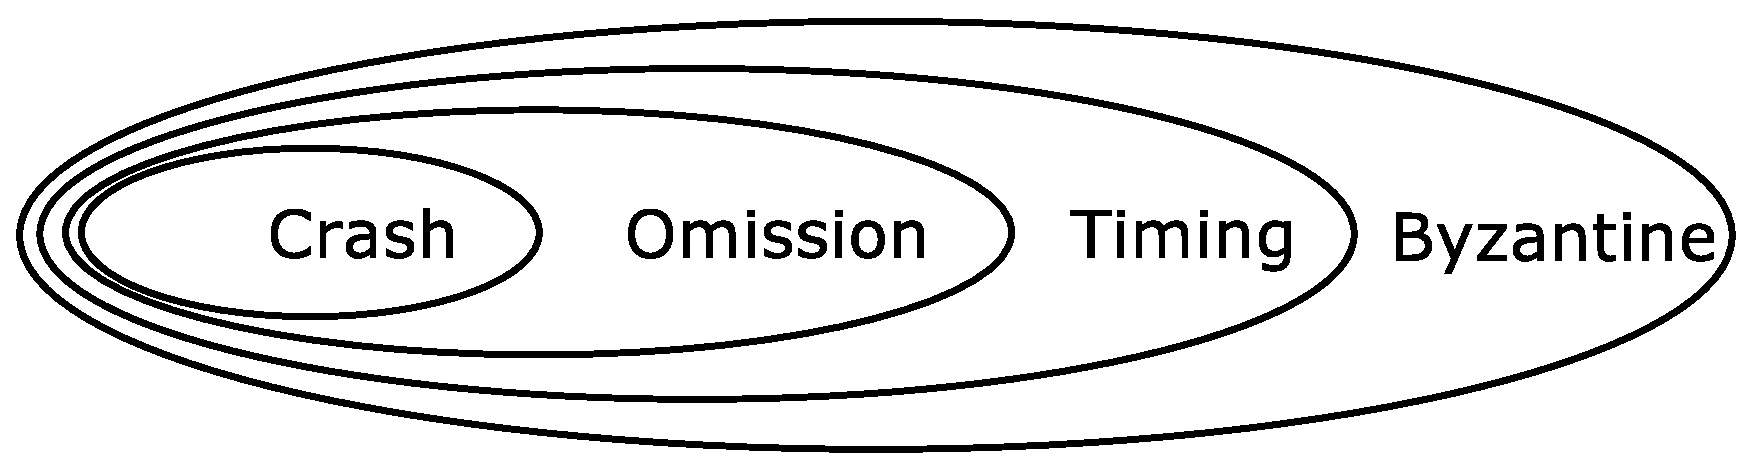
\includegraphics[width=13cm]{conteudo/capitulos/figuras/classificacao_falhas.eps}
  \caption{Classificação de falhas}
  \label{fig:fault-classification}
\end{figure}

Projetamos sistemas distribuídos tolerantes a falhas para fornecer um serviço confiável e
contínuo, apesar das falhas de alguns de seus componentes. Um mecanismo básico utilizado
na construção é o \emph{detector de falhas}, que a grosso modo, fornece algumas
informações sobre as réplicas defeituosas. Em ambientes assíncronos, a informação de falha
normalmente é dada através de uma lista de suspeitas, que nem sempre estão atualizadas ou
corretas. Um detector de falhas pode levar um longo tempo para suspeitar de uma réplica
que deixou de funcionar e pode erroneamente suspeitar de uma réplica correta, na prática
isto pode ser devido à perda de mensagens e/ou atrasos \cite{chandra96, chen02}.


\section{Modelo Operacional}

Para facilitar a construção de uma aplicação que utiliza o modelo de replicação ativa,
esse trabalho emprega uma arquitetura separada em camadas. Essa divisão visa facilitar
a resolução do problema, mitigar os erros e maximizar a compreensão dos experimentos.

Em inglês, duas palavras são comumente utilizadas para se falar de divisão em camadas:
\emph{tier} e \emph{layer}. Ao falar em \emph{layers}, normalmente pensa-se em separações
lógicas, em como organizar o código da aplicação de maneira a diminuir o acoplamento
entre diferentes partes do código e evitar que mudanças em um lugar afetem outros. Já a
divisão em \emph{tiers} visa as separações físicas entre partes do sistema
\cite{caelum11}.

\subsubsection{Tiers}

Para concepção do presente trabalho, supomos uma aplicação Web, conforme ilustrada na
\autoref{fig:tiers}, utilizando um \emph{middleware} que implementa o modelo de replicação
ativa. A função principal desempenhada por esse \emph{middleware} de replicação é
gerenciar o estado da aplicação, executando as requisições dos clientes através de uma
abstração de uma \emph{máquina de estados replicada} \cite{schneider90}. Essa abstração é
implementada utilizando o algoritmo Paxos \cite{lamport98}.

\begin{figure}[ht]
  \centering
  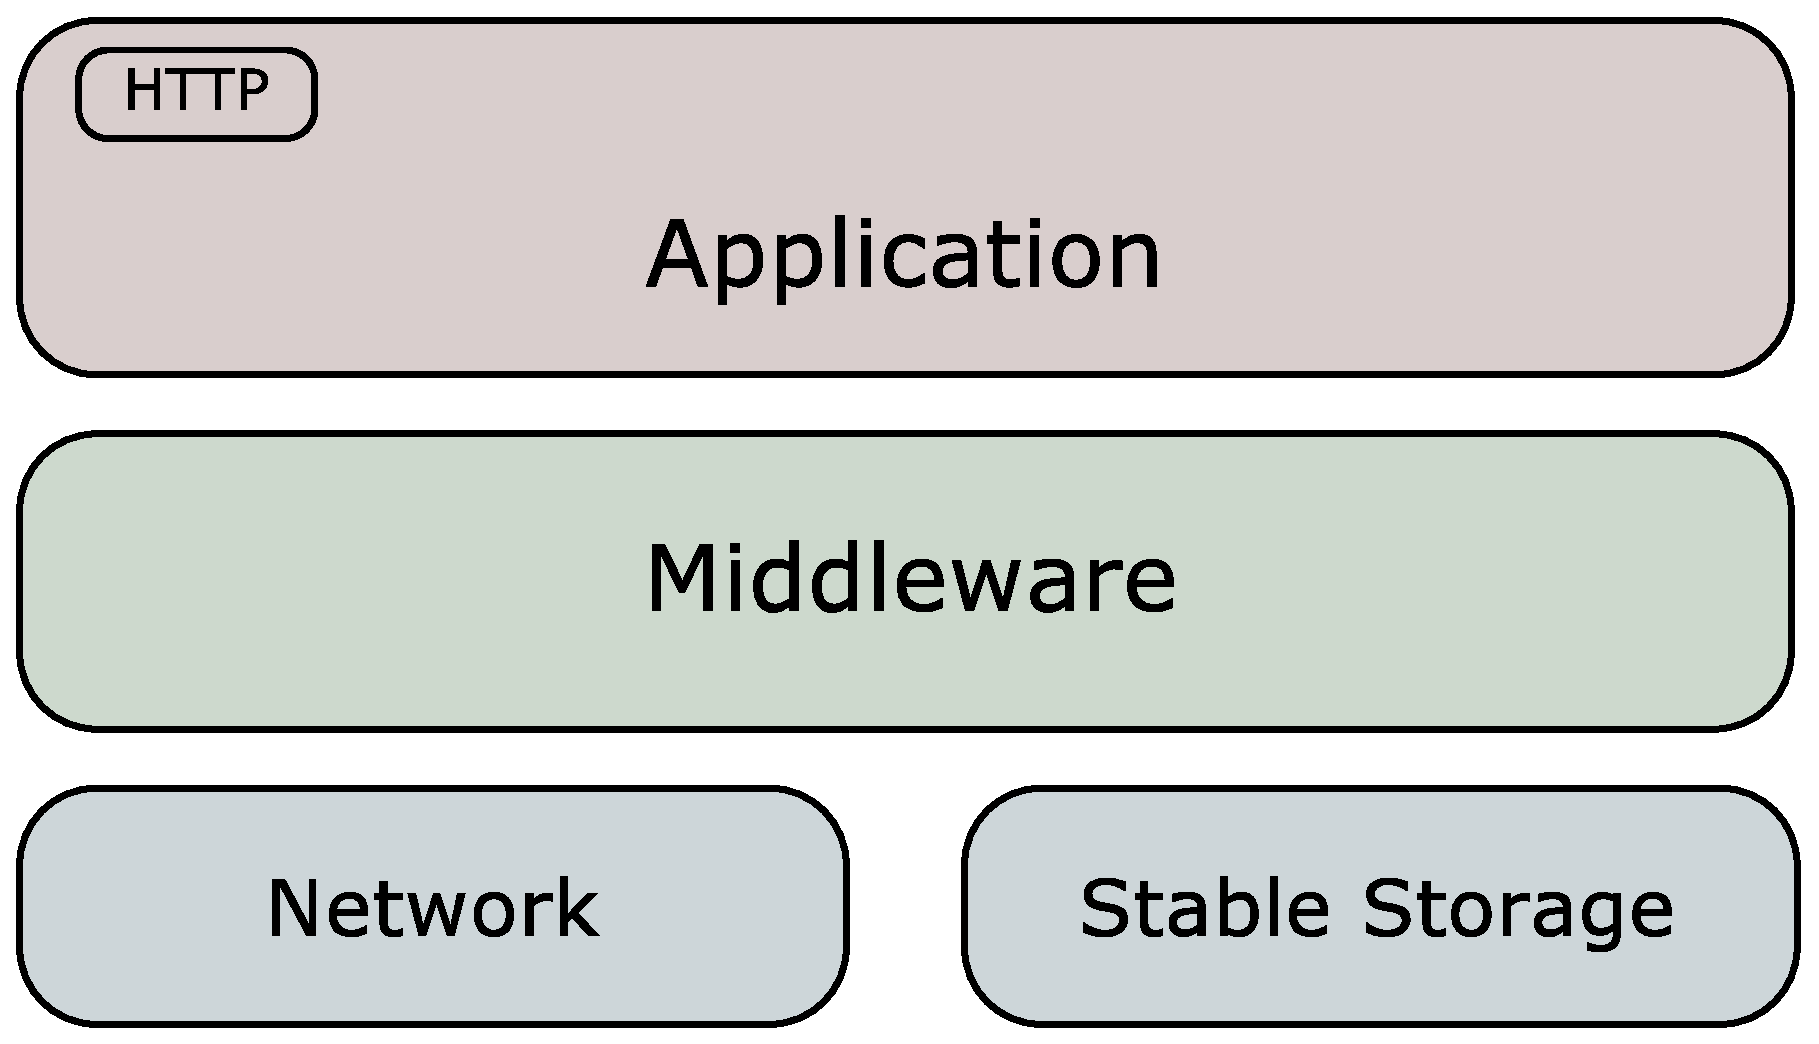
\includegraphics[width=12cm]{conteudo/capitulos/figuras/block-simple.eps}
  \caption{Separação em \emph{tiers}}
  \label{fig:tiers}
\end{figure}

Supomos que a uma aplicação que use replicação ativa o faz na forma de um servidor que
atende \emph{requisições} de \emph{clientes}. Esses clientes não têm conhecimento de como
as requisições são executadas. As réplicas recebem essa requisições e as processam de forma
a manter a consistência do estado replicado (compartilhado). Cada uma dessas requisições
executa o equivalente a uma chamada de função no contexto do estado da aplicação. Se a
função subjacente altera o estado, esta é uma \emph{requisição de escrita} e deve ser
difundida e ordenada entre todas as réplicas antes de ser executada. Caso a função
subjacente não altere estado, esta é uma \emph{requisição de leitura} e pode ser executada
localmente sem coordenação entre as réplicas.

\subsubsection{Layers}

Do ponto de vista da estruturação física para suportar a aplicação, supomos um conjunto de
réplicas que é gerenciada por um servidor balanceador de carga, usado para melhorar o
desempenho de serviços Web distribuindo requisições entre vários servidores. Todas as
requisições dos clientes passam pelo balanceador de carga, configurado para receber e
rotear as requisições para as réplicas ativas, usando um algoritmo de revezamento circular
(\emph{round-robin}), como ilustrado na \autoref{fig:layers}.

\begin{figure}[ht]
  \centering
  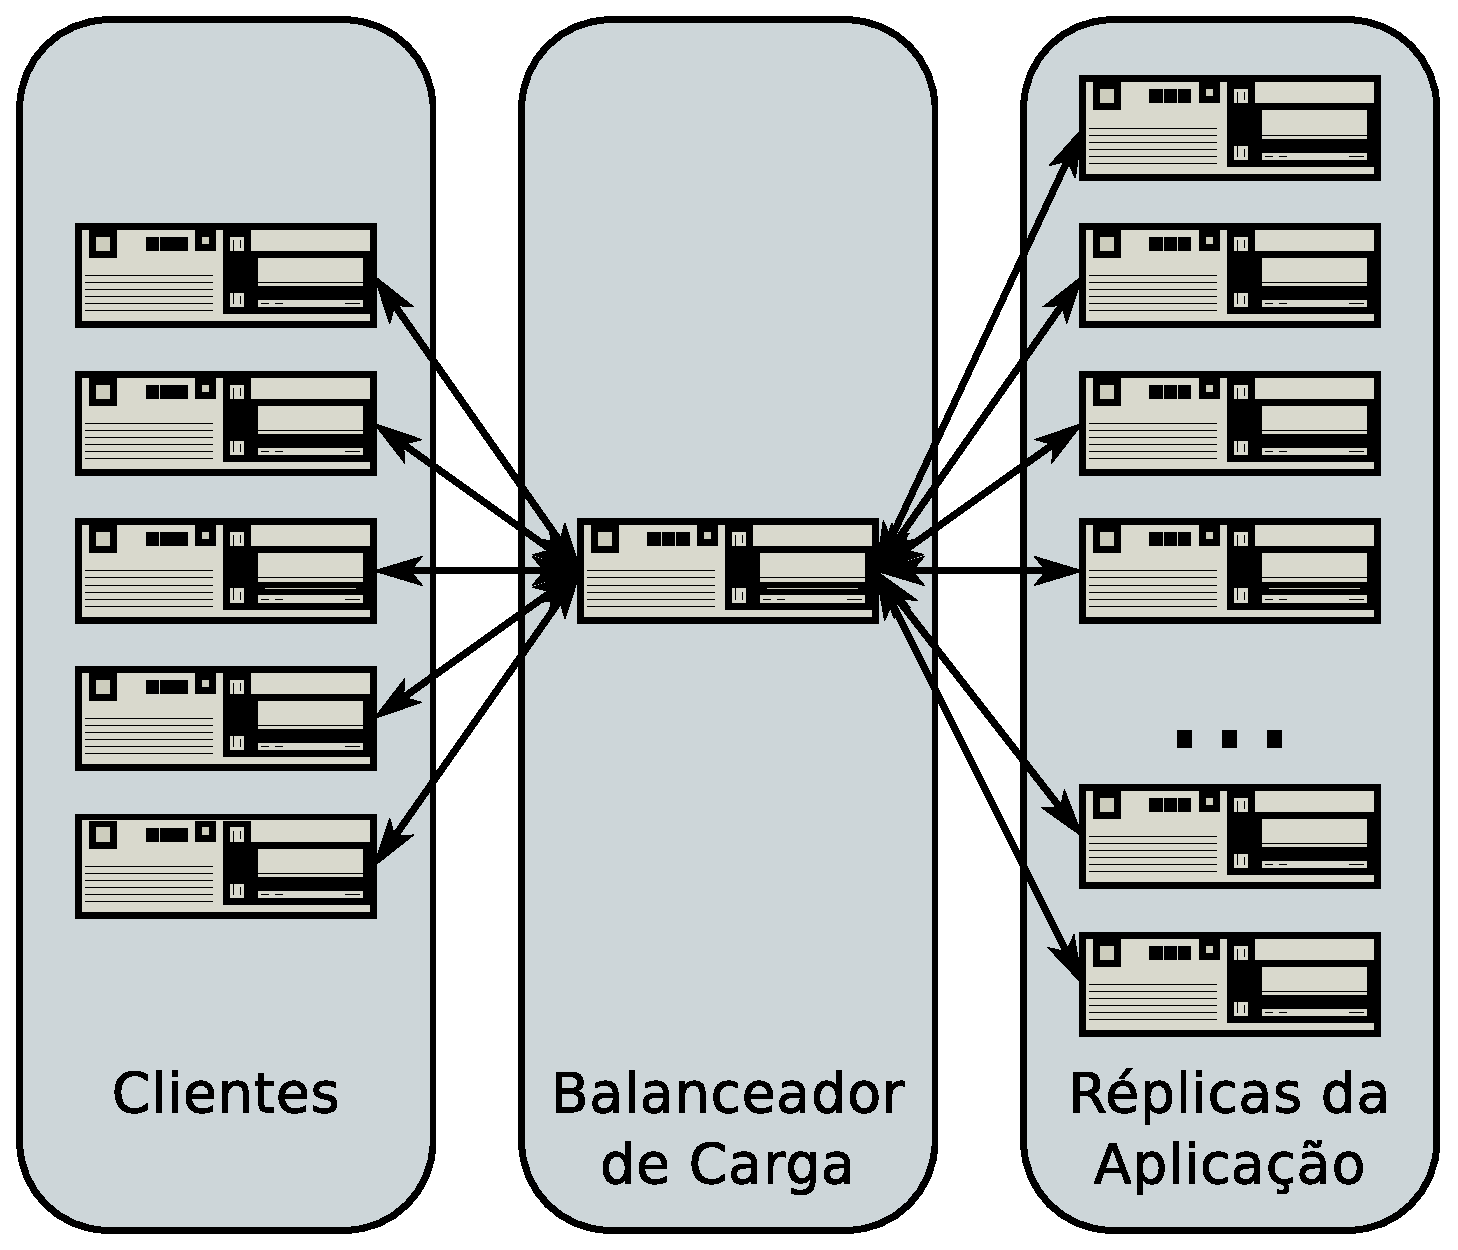
\includegraphics[width=10cm]{conteudo/capitulos/figuras/layers.eps}
  \caption{Separação em \emph{layers}}
  \label{fig:layers}
\end{figure}

O balanceador de carga monitora as réplicas para tentar detectar quando a aplicação está
disponível. Assim que uma réplica está disponível ela passa a receber requisições roteadas
pelo balanceador de carga. O monitoramento é realizado através de pequenos pacotes
\emph{keepalive} que são enviados para cada réplica do aglomerado. Todos os componentes
estão conectados através de um \emph{switch} que se comporta como uma canal de perda-justa.


\section{Replicação Ativa}\label{sec:replicacao-ativa}

Em geral, é uma boa ideia replicar serviços ou dados (estado) de uma aplicação. A
replicação é um mecanismo fundamental em sistemas distribuídos, proporciona maior
disponibilidade e ajuda a equilibrar a carga entre componentes, o que potencialmente
resulta em melhor desempenho \cite{tanenbaum07}. O acesso a serviços ou dados replicados
deve ser transparente para o usuário, ele deve ser realizado da mesma forma que o faria
como se não houvesse replicação. A consistência dos dados replicados deve ser garantido
automaticamente pelas réplicas e mesmo que mais de uma réplica responda a uma requisição,
apenas uma resposta deve ser entregue ao usuário final.

A criação de um grupo de réplicas minimiza a percepção de falhas de um cliente que acessa
um estado compartilhado. Entretanto, para que o grupo de réplicas seja transparente para
aplicação cliente, é preciso adotar uma estratégia de replicação a fim de coordenar as
réplicas preparando-as para que, no momento que ocorrer uma falha, uma réplica possa dar
continuidade ao processamento do sistema~\cite{jalote94}. Existem duas técnicas seminais
de replicação de processos: a \emph{replicação ativa} e a \emph{replicação passiva}
\cite{jalote94}. Esses modelos de replicação são capazes de tolerar falhas de maneira
transparente para o cliente, na ativa a escrita é garantida nas réplicas e na passiva a
escrita ocorrerá mais cedo ou mais tarde (futura).

Na replicação ativa \cite{coulouris11, guerraoui97} ou replicação por máquina de estados
\cite{schneider90}, os processos replicados funcionam como máquinas de estado
deterministas, ou seja, o estado atual é determinado única e exclusivamente por um estado
inicial e uma sequência de transições. Desta forma, se os processos replicados recebem a
mesma sequência de transições eles atingirão estados idênticos.

Cada operação que altera o estado de uma réplica (requisição de escrita) é executada de
maneira determinista no conjunto de réplicas, ou seja, todas as réplicas recebem e
processam a mesma sequência de requisições, conforme ilustrado na
\autoref{fig:write-replication}.

\begin{figure}[htbp]
  \centering
  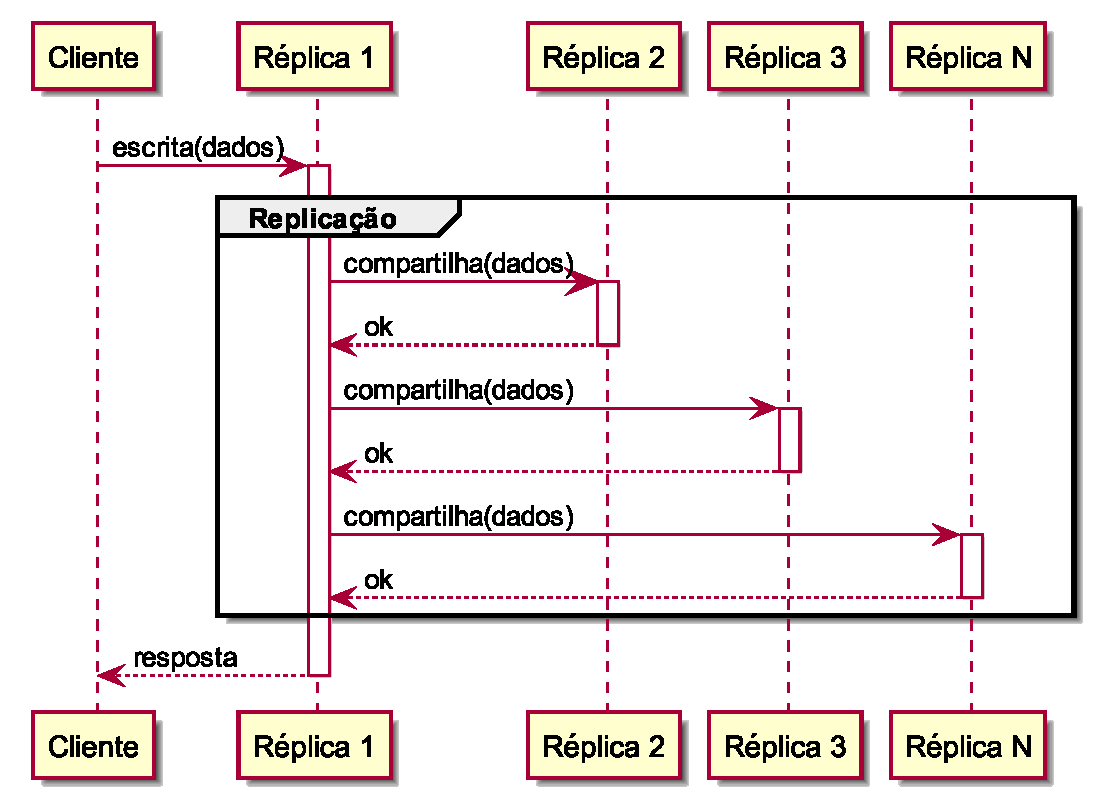
\includegraphics[width=12cm]{conteudo/capitulos/figuras/escrita.eps}
  \caption{Requisição de escrita}
  \label{fig:write-replication}
\end{figure}

A propagação das requisições de mudança no conjunto de réplicas garante a sincronização
consistente global do estado, pois é replicando a atualização de estado sofrida por uma
réplica em todas as outras réplicas que uma requisição de leitura pode ser executada
localmente em qualquer réplica com a certeza do mesmo resultado. A
\autoref{fig:read-replication} ilustra esse cenário, repare que não existe propagação da
requisição para outras réplicas, a requisição e processada localmente.

\begin{figure}[htbp]
  \centering
  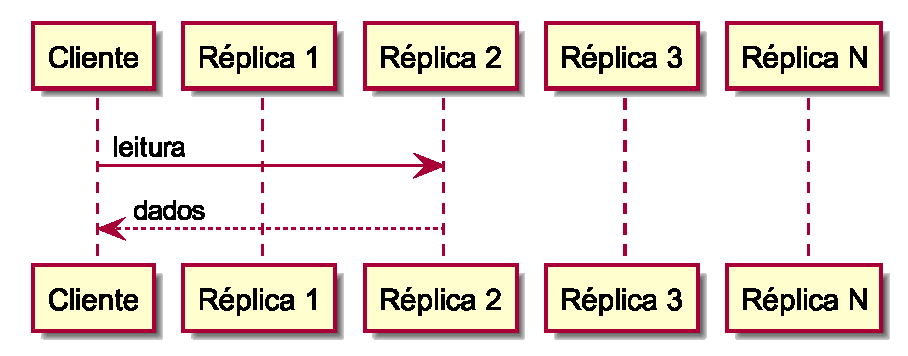
\includegraphics[width=10cm]{conteudo/capitulos/figuras/leitura.eps}
  \caption{Requisição de leitura}
  \label{fig:read-replication}
\end{figure}

Não é necessário modelar o funcionamento de uma aplicação que use replicação ativa como
uma máquina de estados explícita, basta considerar as funções da aplicação que mudam o
estado como transições. As funções que não mudam o estado não têm correspondência na
abstração de máquina de estados, sendo simples consultas ao estado armazenado e não exigem
ordenação.

Uma desvantagem da replicação ativa é que por requerer réplicas deterministas ela
restringe o uso de múltiplos fluxos de execução (\emph{multithreading}) e outros
mecanismos que podem causar indeterminismos, mas que podem melhorar o desempenho. O
requisito de ordem total pode ser relaxado se as requisições dos clientes forem
comutativas ou idempotentes. Para um sistema $f-$tolerante a falhas, são necessários $f +
1$ réplicas ativas para garantir progresso da aplicação \cite{jalote94, lamport10}.
Requisições de escrita encarecem a aplicabilidade desse modelo, pois precisamos escrever
em um número grande o suficiente de réplicas de tal forma que a escrita não seja
esquecida.

Replicação ativa consistente é uma tarefa complicada e cara porque no modelo computacional
adotado não há uma ideia de relógio global compartilhado. Ou seja, processos em máquinas
diferentes têm sua própria ideia do que é o tempo e como ele passa, logo não podem
determinar com certeza se alguma das outras réplicas estão defeituosas. Para garantir a
consistência, as réplicas devem executar a mesma sequência de eventos, dessa forma é
possível manter o estado análogo em qualquer réplica, mesmo que o mesmo evento em máquinas
diferentes seja processado em momentos distintos \cite{tanenbaum07}. Ordenar as
requisições de forma única, na presença de falhas, é equivalente a resolver o problema de
consenso \cite{chandra96}.


\section{Paxos}\label{sec:paxos}

O algoritmo Paxos \cite{lamport98} é uma solução completa para replicação ativa usando
consenso. Paxos é destinado ao modelo assíncrono de computação com falha-e-recuperação que
utiliza detectores de falha imperfeitos. Em particular, ele garante que o estado de
nenhuma réplica irá divergir do das demais, mesmo na presença de falhas e de comportamento
assíncrono de processamento e canais de comunicação.

Paxos emprega um conjunto de protocolos baseados em quórum para atualizar os dados
replicados em um grupo. O objetivo do algoritmo é coordenar as réplicas para que todas
tenham o mesmo estado \cite{cachin11}. Para garantir o progresso e correção do algorítimo,
as seguintes propriedades são destacadas:

\begin{itemize}
  \item Validade Uniforme: se um processo decide $v$ então algum processo anteriormente
    propôs $v$.
  \item Acordo: não existem dois processos corretos que decidem valores diferentes.
  \item Encerramento: Se todos os processos corretos propõem um valor, então mais cedo ou
    mais tarde, eles serão decididos.
\end{itemize}

Por utilizar um mecanismo baseado em quórum, o algoritmo não depende de que todas as
réplicas estejam ativas para garantir que a escrita seja durável. Entenda por durabilidade
\footnote{Semelhante a propriedade ACID definida em transações de banco de dados
\cite{haerder83}} que uma vez que a transação foi confirmada, ela permanecerá assim, mesmo
em caso de falhas ou erros. Ou seja, os dados foram gravados em memória não-volátil.

\subsection{Algoritmo Básico}\label{subsec:algoritmo_basico}

Em Paxos os processos no sistema são agentes reativos que podem assumir vários
papéis: \emph{proponente} (\emph{proposer}) que pode propor valores, \emph{receptor}
(\emph{acceptor}) que escolhe um único valor ou \emph{aprendiz} (\emph{learner}) que
aprende o valor escolhido. Para resolver o consenso, agentes do Paxos executam várias
\emph{rodadas} (\emph{rounds}), onde cada rodada possui um \emph{coordenador}
(\emph{coordinator}) e é unicamente identificado por um inteiro positivo, o \emph{número
de rodada}. Proponentes enviam a sua \emph{proposta} para o coordenador que tenta alcançar
consenso sobre a proposta em uma rodada, sendo que cada proposta corresponde a uma ou mais
requisições de escrita da aplicação sendo replicada.

O coordenador é responsável por essa rodada e executa um número definido de passos de
comunicação para garantir que a decisão tomada nessa rodada seja aceita pelos demais
processos, ou seja, um consenso. Este agente de Paxos é capaz e decidir, após aplicar uma
regra local, se outras rodadas tiverem sucesso ou não. A regra local do coordenador é
baseada em quóruns de receptores e exige que pelo menos $\lfloor n/2 \rfloor + 1$
receptores façam parte de uma rodada, onde $n$ é o número total de receptores na
aplicação \cite{lamport98}.

Cada rodada acontece em duas fases, com dois passos cada, como ilustrado na
\autoref{fig:fases-paxos}:

\begin{itemize}
  \item Na Fase 1a o coordenador envia uma mensagem convidando todos os receptores a
    participar de uma rodada $r$. Um receptor aceita o convite apenas se ele não aceitou
    participar de uma rodada $s \geq r$. Caso contrário, ele ignora o convite.
  \item Na Fase 1b todo receptor que aceitou o convite responde ao coordenador informando
    a última proposta votada por esse receptor e a rodada em que esse voto ocorreu, ou
    \textsl{null} se ele nunca votou.
  \item Na Fase 2a, se o coordenador da rodada $r$ recebeu respostas de um quórum de
    receptores, ele analisa o conjunto de respostas recebidas e escolhe uma proposta $p$
    que foi ou que poderia ter sido decidida em rodadas com número menor que $r$. Ele
    então pede a esses receptores para votar nessa proposta, ou caso ela seja
    \textsl{null}, para votar em uma das propostas feitas pelos proponentes.
  \item Na Fase 2b, após receber um pedido para votar do coordenador, receptores votam na
    proposta sugerida se eles não votaram em nenhuma rodada $s \geq r$. Os receptores
    votam enviando o número de rodada e a proposta aos aprendizes.
  \item Finalmente, um aprendiz descobre que uma proposta $p$ foi escolhida se ele receber
    mensagens da Fase 2b de um quórum de receptores, todos votado em $p$ na mesma rodada
    $r$.
\end{itemize}

\begin{figure}[htbp]
  \centering
  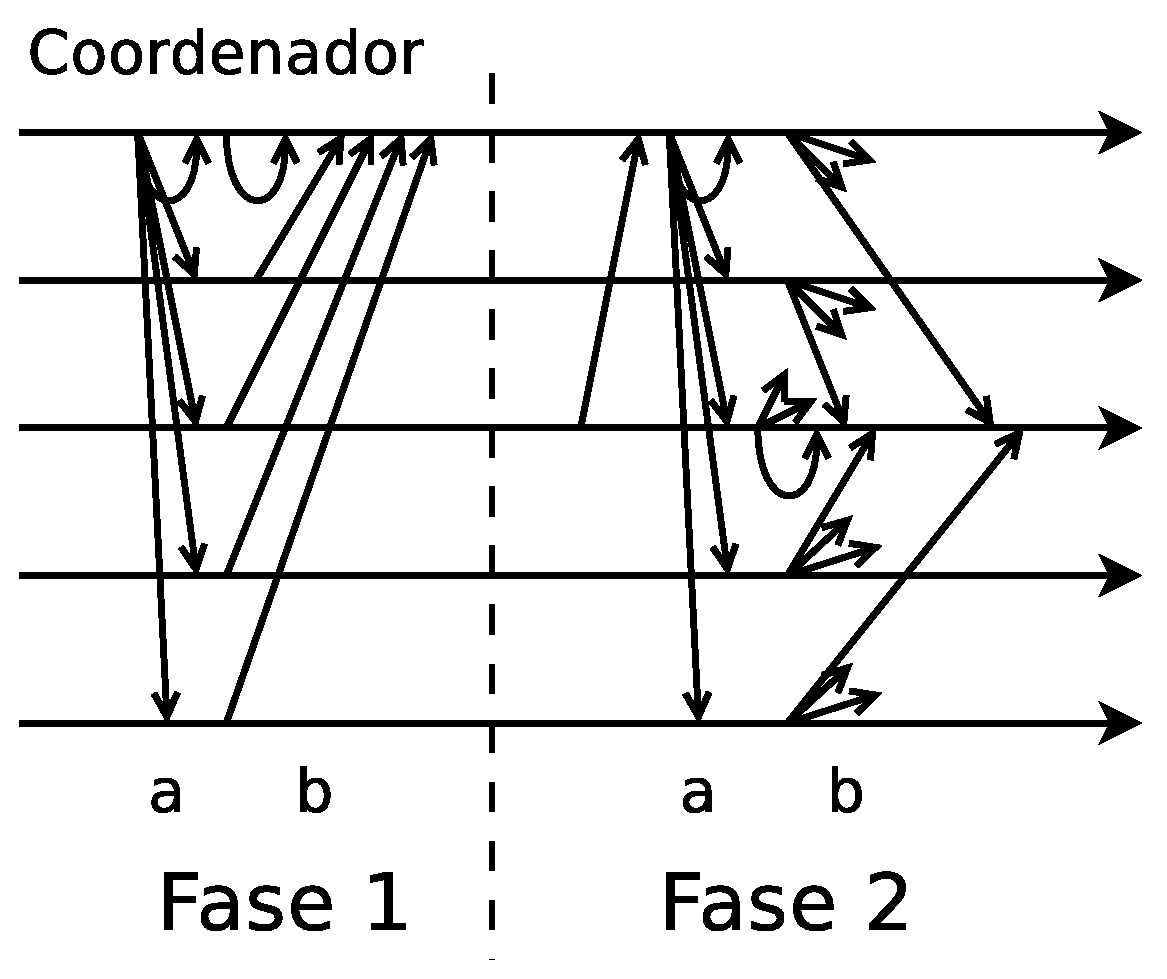
\includegraphics[width=9cm]{conteudo/capitulos/figuras/paxos.dia.eps}
  \caption{Paxos}
  \label{fig:fases-paxos}
\end{figure}

Cada rodada corresponde à decisão de uma proposta apenas. Porém Paxos define também uma
forma de entregar um conjunto de requisições de escrita totalmente ordenadas. A ordem de
entrega dessas requisições é determinada pela sequência dos inteiros positivos, tal que
cada inteiro corresponde uma \emph{instância} de consenso. Cada instância $i$ terá um
valor decidido, que corresponde a $i$-ésima requisição (ou conjunto ordenado de
requisições) a ser executada na sequência de requisições. Cada instância de consenso é
independente das demais e várias instâncias podem estar em curso ao mesmo tempo.

Como Paxos é definido no modelo falha-e-recuperação assíncrono, esse algoritmo exige que
os agentes armazenem estado em memória não volátil \cite{lamport06a}. Esse estado é
composto por um registro das instâncias iniciadas, os números de rodadas usados e as
propostas feitas e votadas, entre outros dados. De forma resumida, o coordenador escreve
na memória persistente na Fase 1a e os receptores o fazem nas Fases 1b e 2a. Não há a
necessidade de que a proposta decidida seja registrada para garantir a correção do
algoritmo, mas isto é normalmente feito para acelerar a recuperação. A escrita de dados em
memória persistente faz parde do caminho crítico de desempenho da execução das duas fases
do algoritmo Paxos. Logo, dependendo do custo de comunicação de rede, esse é o principal
gargalo de desempenho para a execução de Paxos.

Em Paxos, qualquer processo pode agir como o coordenador de uma rodada enquanto ele seguir
a regra para escolher uma proposta coerente como o resultado das rodadas anteriores na
Fase 2a. A escolha do coordenador e a decisão de iniciar uma nova rodada de consenso são
feitas com base em algum mecanismo de temporização, uma vez que Paxos supõe um modelo
computacional parcialmente síncrono para garantir progresso (\emph{liveness}).
Especialmente, a todo momento deve existir apenas um coordenador ativo para garantir que o
algoritmo progrida. Se dois ou mais processos iniciam agentes coordenadores, o algoritmo
pode travar enquanto estes múltiplos coordenadores competem pela atenção dos receptores
com números de rodada que crescem rapidamente. Por esta razão, o progresso do algoritmo
depende de um procedimento de seleção de coordenador. Este procedimento não precisa ser
perfeito. A correção do algoritmo nunca é comprometida se zero ou mais coordenadores
estiverem ativos ao mesmo tempo. Porém, o procedimento de seleção de coordenador deve ser
robusto o suficiente para garantir que apenas um único coordenador esteja ativo a maior
parte do tempo.

\subsection{Recuperação}

Uma consideração em relação ao funcionamento típico de Paxos é o que acontece
quando uma réplica inicia depois que o sistema já está operando ou quando reinicia após
uma falha prolongada. Esse caso não é explicitamente definido na descrição clássica de
Paxos, porém o algoritmo permite que um número arbitrário de rodadas aconteçam
\emph{antes} ou \emph{depois} que o consenso seja alcançado \cite{lamport98}. Dessa forma,
podemos supor um mecanismo de recuperação simples onde uma réplica que ficou fora de
operação por algum tempo atualiza o seu estado pela decisão sucessiva das instâncias de
consenso que ela não tem conhecimento. Esse mecanismo é apropriado para pequenas
interrupções, como a perda de algumas mensagens ou uma falha transiente. Porém, caso uma
réplica tenha um grande estado para atualizar esse procedimento pode ter impacto adverso
no desempenho do sistema.

Para exemplificar o possível impacto cenário de recuperação, vamos supor as seguintes
propriedades relacionadas a atualização de uma réplica desatualizada:

\begin{itemize}
  \item Consistência: Uma réplica desatualizada $r$ volta a computação após $n$ rodadas de
    consenso, onde $n$ é um número arbitrariamente grande. Se $r$ aplicar as $n$ decisões
    de consenso sucessivamente atingirá o mesmo estado das demais réplicas.
  \item Volatilidade do estado: Se o número de rodadas de consenso $n$ muda em uma
    velocidade maior que a réplica desatualizada $r$ consegue atualizar seu estado, $r$
    estará sempre desatualizada \cite{vilaca09}.
\end{itemize}

Baseado nessas propriedades de consistência e volatilidade não podemos afirmar nada com
relação ao tempo de recuperação de estado de uma réplica. O mecanismo de recuperação por
aplicação de decisões de consenso é ineficiente quando uma réplica possui um estado muito
antigo. Para atendermos eficientemente este cenário, precisamos de uma nova política de
recuperação. Uma alternativa é transferir para a réplica desatualizada o estado de uma
réplica atualizada, dessa forma supriremos a lacuna de desatualização substituindo por
completo o estado desatualizado por um atualizado, semelhante a ideia de um transplante.

\subsection{Estado persistente}\label{subsec:estado_persistente}

Para satisfazer as propriedades de consenso no modelo falha-e-recuperação assíncrono é
preciso utilizar um mecanismo capaz de gravar dados de forma persistente (não-volátil).
Dessa forma, após um período de instabilidade uma réplica é capaz de recuperar suas
decisões de consenso tomadas anteriormente para continuar participando corretamente do
protocolo. A cada fase do algoritmo acontecem dois acessos a disco, conforme ilustrado na
\autoref{fig:fases-paxos-acesso-disco}

\begin{figure}[htbp]
  \centering
  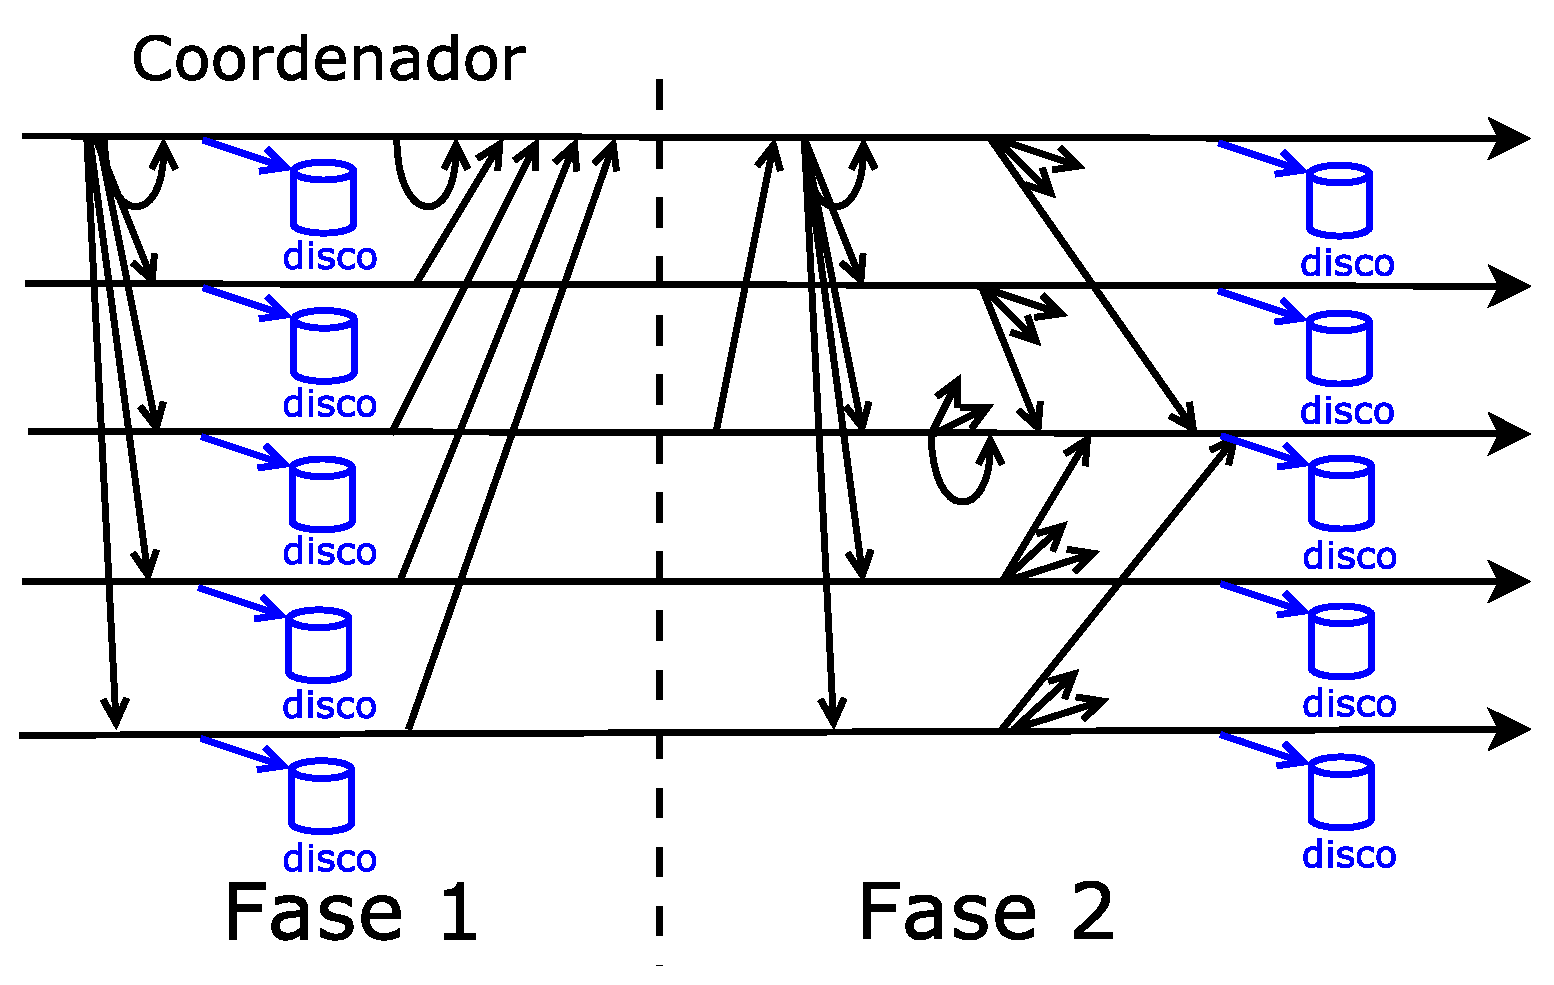
\includegraphics[width=9cm]{conteudo/capitulos/figuras/fases-paxos-acesso-disco.eps}
  \caption{Acesso a disco em Paxos}
  \label{fig:fases-paxos-acesso-disco}
\end{figure}

\begin{itemize}
  \item Na Fase 1, após receber um convite do coordenador para participar da rodada $r$,
    todo receptor que aceitou o convite, escreve $r$ em disco.
  \item Na Fase 2, toda a proposta $p$ que consegue estabelecer consenso em $r$ é
    escrita em disco. Ao final de cada rodada, foi persistido em disco o par (rodada,
    decisão).
\end{itemize}

Operações de persistência durável é custosa e tem grande potencial para reduzir o
desempenho do algoritmo. Por exemplo, considere que cada operação de escrita em disco leva
cerca de $1ms$ para ser concluída e que uma rodada de Paxos, pelo menos, requer duas
escritas em memória estável, acabamos de adicionar uma latência de $2ms$ em todas as
rodadas de consenso. \citeonline{aguilera00} propõem a combinação de réplicas com
diferentes graus de uso de memória persistente para diminuir o custo do armazenamento dos
dados. Essa proposta, através de vários teoremas, mostra que se o número de processos que
nunca falham é maior que o número de processos que eventualmente permanecem defeituosos ou
falham e se recuperam infinitamente, então o consenso pode ser resolvido sem armazenamento
persistente.

Esse trabalho apresenta a resolução de consenso nesse modelo com um número variável de
réplicas com memória persistente, desde que seja sempre possível entrar em contato com
uma réplica que use memória persistente ou com uma réplica sem memória persistente que
nunca falhe. Nossa proposta de replicação aplica-se para o algoritmo Paxos, determinando
que os quóruns responsáveis pelo consenso sejam sempre compostos por réplicas que usam
memória persistente.


\section{Treplica}\label{sec:treplica}

Treplica se situa a meio caminho entre flexibilidade de baixo nível de um sistema de
comunicação em grupo \cite{birman93} baseado em sincronia virtual \cite{friedman96,
birman05} e os vastos recursos de processamento de dados de um SGBD. A principal
característica de Treplica é a ideia de se apresentar ao programador como uma abstração de
programação unificada para replicação e persistência, propondo o uso de consenso
\cite{barborak93} como a fundação para a construção dessa ferramenta.

Treplica foi projetada para prover uma forma simples e orientada a objetos de se construir
aplicações altamente confiáveis. Essas aplicações podem se estender ao sistema inteiro ou
se restringir à subsistemas onde o desempenho, consistência e confiabilidade são cruciais.
Para alcançar esse objetivo, Treplica decompõe o problema de se implementar replicação em
componentes com interfaces simples e bem definidas.

Dessa forma, um desenvolvedor que deseje implementar uma aplicação distribuída não precisa
pensar em termos de processos, mensagens e falhas. Ao invés disso, ele pensa sobre a
execução das operações da aplicação, transições de uma máquina de estados replicada, que
são disparadas por eventos disponibilizados através de uma fila persistente assíncrona
\cite{vieira-tr10b}. A \autoref{fig:treplica} mostra a interface destes componentes e sua
relação com a aplicação e entre si.

\begin{figure}[ht]
  \begin{center}
    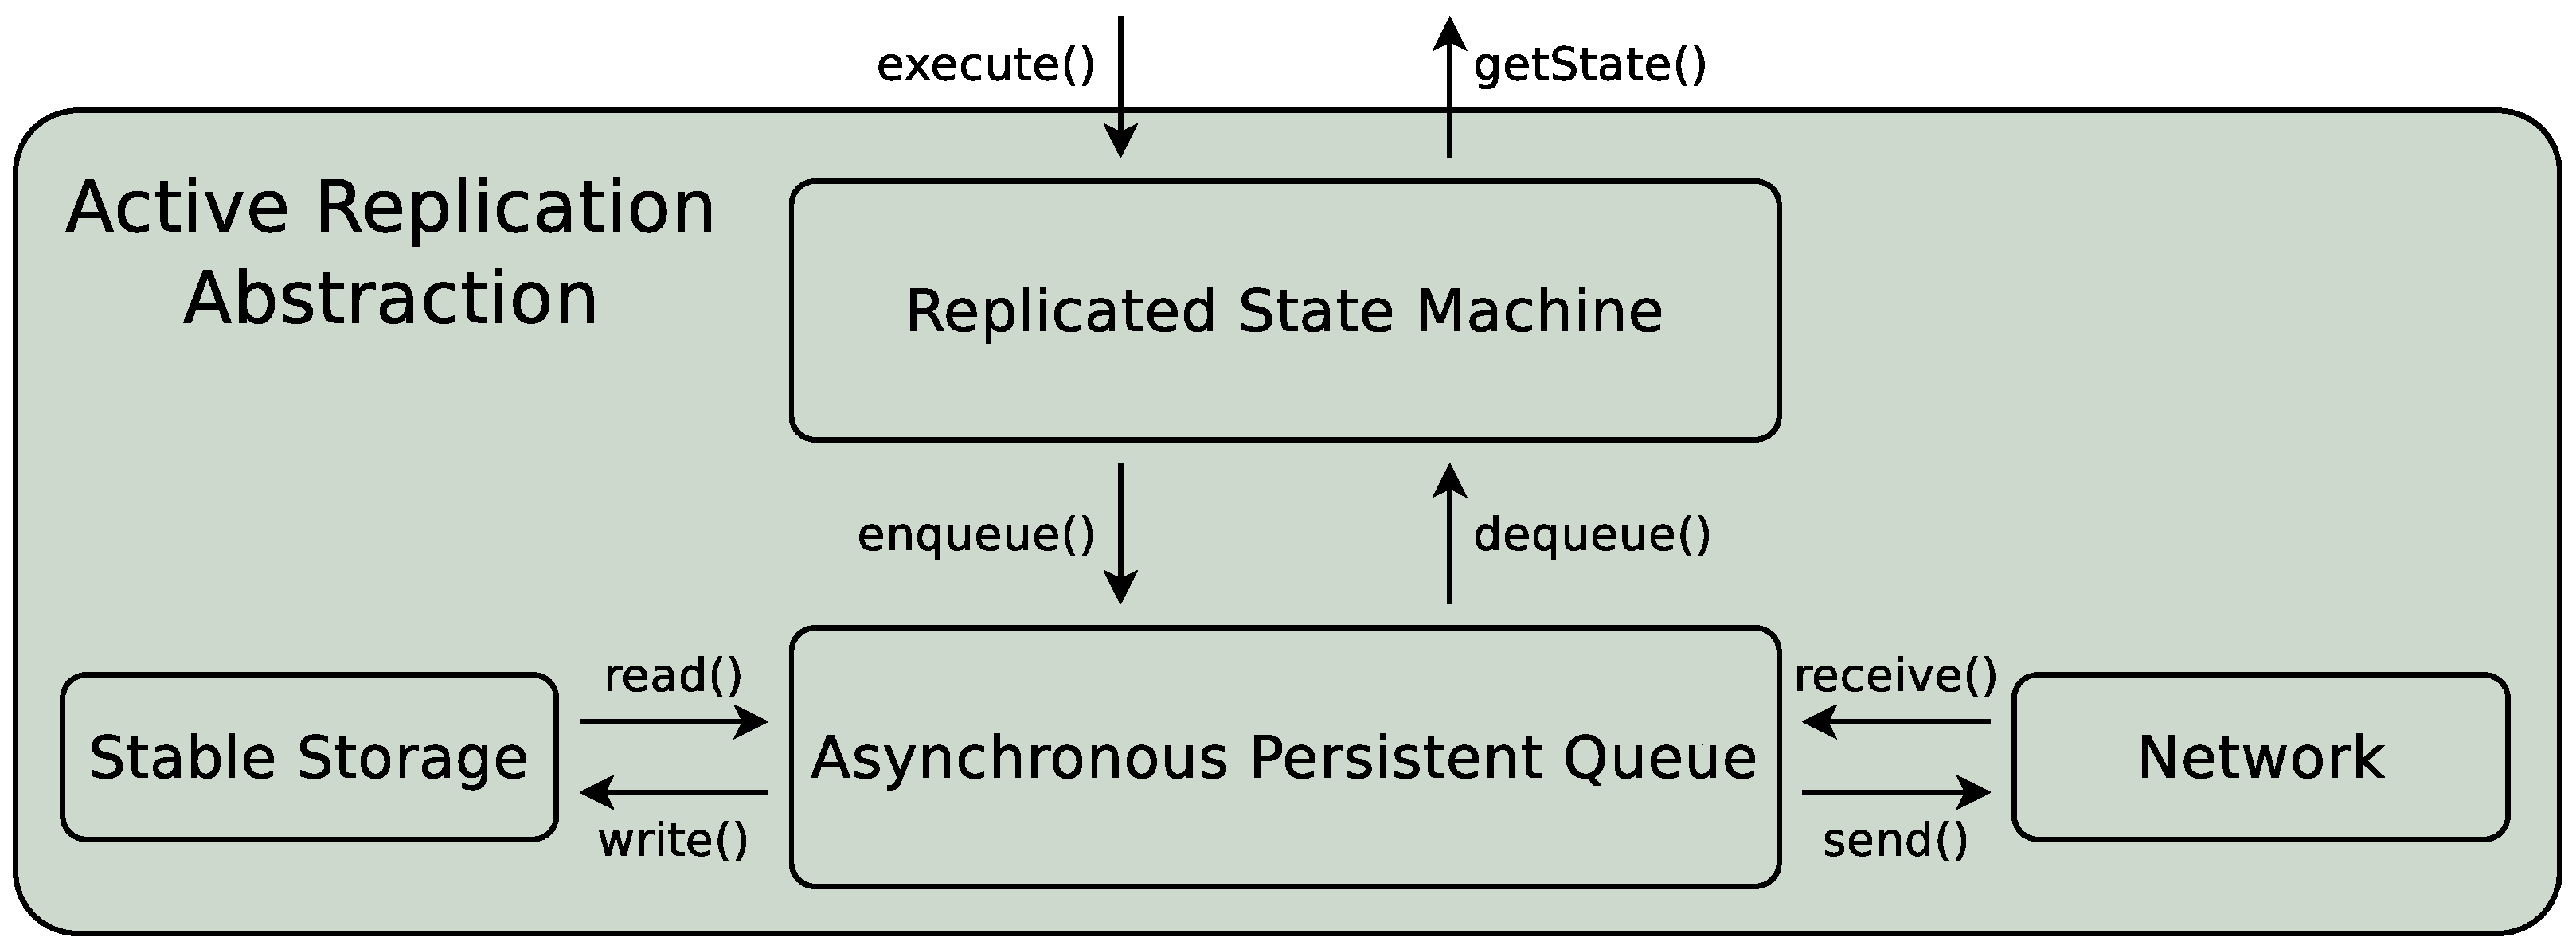
\includegraphics[width=14cm]{conteudo/capitulos/figuras/treplica.eps}
  \end{center}
  \caption{Componentes para replicação}
  \label{fig:treplica}
\end{figure}

A principal decisão de projeto por trás de Treplica é que o programador pode considerar a
sua aplicação como não tendo estado persistente, ficando a durabilidade da mesma garantida
pela biblioteca. Essa decisão é suportada pela observação que os mesmos requisitos de
replicação ativa podem ser usados para prover um mecanismo simples e poderoso de
persistência.

A replicação ativa exige que a aplicação execute ações que modificam o seu estado de forma
determinista. Essas ações são então propagadas, na mesma ordem, para todas as réplicas de
um serviço que as reexecutam localmente. Dentro dessa organização, as ações não são apenas
enviadas para as outras réplicas, mas arquivadas em memória estável \cite{birrel87}. Dessa
forma, é possível se recuperar de uma falha reexecutando o arquivo de ações. O
determinismo garante que após cada recuperação a aplicação reiniciará com o mesmo estado
que possuía antes da falha. Por razões de eficiência, a aplicação deve caber inteiramente
em memória principal, pois a biblioteca não armazena a aplicação em si, apenas mudanças de
estado.

A máquina de estados replicada provê uma abstração da operação de qualquer aplicação
determinista. Ela permite a manutenção do estado da aplicação estipulando uma interface
simples para consultar e modificar esse estado. Esse componente é acessado diretamente
pela aplicação que usa os seus serviços para armazenar, replicar e persistir o seu estado.
Todas essas operações são realizadas de forma transparente e não exigem intervenção por
parte do usuário desse componente.

A fila persistente assíncrona é uma abstração de uma fila de objetos persistentes e
tolerante a falhas. Ela representa um registro ordenado de objetos enviados a um grupo de
processos, que é garantidamente disponível mesmo se todos os processo deste grupo falhem.
Ela pode ser usada como um registro persistente dos eventos que disparam transições na
máquina de estados distribuída e é implementada usando algum mecanismo de difusão ordenada
de mensagens, como Paxos descrito na \autoref{sec:paxos}.


\section{Reconfiguração}\label{sec:reconfiguracao}

O processo de modificar o conjunto de réplicas que compõem o sistema chama-se
\emph{reconfiguração}. Alterar o número de réplicas participantes de uma aplicação que
utiliza o modelo de replicação ativa não é uma tarefa trivial pois a informação de
\emph{cardinalidade} do conjunto de réplicas é relevante para o mecanismo de replicação
gerenciar a consistência do estado compartilhado. Segundo \citeonline{lamport10}
reconfigurar é custoso, pois o algoritmo  Paxos trabalha com consenso e para que uma
rodada de consenso ocorra é preciso que o número de réplicas participantes seja claramente
definido. Isso obriga que cada expansão ou redução do grupo de réplicas seja precedido de
reconfiguração.

Paxos trabalha com protocolos baseados em quóruns, então a retirada de uma réplica da
computação sem a devida reconfiguração afeta diretamente o funcionamento correto do
algoritmo que foi projetado para trabalhar com um grupo estático de réplicas
\cite{chandra96, lamport98}, onde não é permitida a entrada e saída de servidores durante
a execução. Essa abordagem não é adequada para sistemas que permanecerão em execução por
um longo tempo, pois limitam a atuação de um administrador, que em tempo de execução, não
pode adicionar máquinas no sistema (para suportar um aumento na carga de processamento) ou
trocar máquinas antigas (para efetuar um reparo no hardware) \cite{alchieri14}. Oferecer
suporte a esses requisitos caracteriza, em sua forma mais simples, um comportamento
elástico que a aplicação deve suportar para refletir mudanças do ambiente operacional
durante o período de execução.

Para formar uma maioria que votou em uma mesma proposta é preciso que o mecanismo de
decisão de consenso conheça o número exato de réplicas em uma determinada rodada. Por
exemplo, caso existam apenas $\lfloor n/2 \rfloor + 1$ potenciais replicas e uma réplicas
$r$ for removido de forma ingênua, a formação legítima de quóruns não é mais possível.
Nesse caso, réplicas corretas serão levadas a 1) suspeitar indevidamente que $r$ falhou,
mas na realidade $r$ não pertence mais ao grupo de réplicas; 2) esperar indefinidamente
por uma resposta de $r$ para determinar a maioria. Essa espera indevida pode impedir a
progresso do algoritmo.

Por outro lado, uma aplicação configurada para executar com $n$ réplicas não pode
adicionar uma nova réplica de forma arbitrária sem ser precedida de reconfiguração. Caso
existam $n + 1$ réplicas ativas, a formação de um quórum que contenha todas as decisões de
consenso pode não ser mais verdade, pois não podemos mais garantir interseção de consenso
no conjunto de réplicas. Dessa forma afetamos diretamente a correção do algoritmo.

Para oferecer o dinamismo necessário na \emph{ampliação} e \emph{redução} de grupos
de réplicas em sistemas distribuídos modernos, \citeonline{lamport10} propõem a criação de
um mecanismo de visões. Nessa proposta uma nova visão $v$ do sistema é criada sempre que uma
réplica $r$ for adicionada ou retirada da computação. Nessa visão $v$, $r$ pode fazer
parte ou não do processamento computacional, dependendo da operação executada. Durante a
execução de uma aplicação, ela pode passar por diferentes visões (configurações) sem
afetar seu progresso e correção, mas sistemas práticos tendem a evitar essa questão de
forma a simplificar a construção de aplicações \cite{chandra07}.

Projetar mecanismos autônomos capazes de realizar reconfiguração, sintonizados para reagir
rapidamente às mudanças do sistema e gerar novas réplicas com base no uso de recursos e
medidas de desempenho, é um assunto atual e relevante para pesquisa. Por outro lado,
estamos preocupados com o impacto inerente de implantar uma nova réplica em um aglomerado
em tempo de execução. Se perceptível tal impacto dificulta a viabilidade das técnicas de
autogestão, porque dependendo do cenário adicionar uma nova réplica pode comprometer o
desempenho de um sistema sobrecarregado \cite{vilaca09}.

Segundo o estudo de \citeonline{vilaca09}, a política de reconfiguração deve levar em
consideração a velocidade das mudanças de estado da aplicação no momento que deseja
reconfigurá-la. Isso  ocorre  pois quando a eficiência da transferência é menor que a
velocidade de mudanças no estado, a nova réplica  nunca receberá o estado mais atual da
aplicação podendo não participar das rodadas atuais de consenso.

Então temos dois problemas em mãos: (1) alterar o numero de réplicas sem violar o
progresso do algoritmo quando remover réplicas e a correção do algoritmo quando adicionar
réplicas. Dessa forma prover uma capacidade elástica preservando a consistência de Paxos;
(2) provisionar réplicas de forma que não comprometa o desempenho, aumentando o suporte
aos picos de acesso, denominados \emph{flash crowds}, existentes na Internet
\cite{tanenbaum07}.


\section{Trabalhos Relacionados}\label{sec:trabalhos-relacionados}

A ideia de se combinar réplicas com diferentes graus de uso de memória persistente no
modelo falha-e-recuperação assíncrono foi formalizada por \citeonline{aguilera00}. Para
esse trabalho supomos a resolução de consenso nesse modelo, utilizando o algotimo Paxos
com um número variável de réplicas que possuem memória persistente. Estabelecemos a forte
premissa que os quóruns responsáveis pelo consenso sejam sempre compostos por réplicas que
usam memória persistente.

Do ponto de vista de engenharia de sistemas, a nossa proposta se assemelha às arquiteturas
de cache distribuídas. Um exemplo notável é o Mencached
\footnote{\url{http://memcached.org/}} que é um repositório de chave/valor. Esse sistema é
usado para armazenar, de forma distribuída pelo aglomerado, dados que podem que a
aplicação faça consultas custosas a um banco de dados centralizado. Usando Mencached o
projetista de aplicação deve modificar o seu programa para registrar as informações úteis
para atender requisições de leitura no cache distribuído. De forma similar, a nossa
proposta procura evitar que seja feito acesso a um recurso nobre, nesse caso as réplicas
votantes. Porém, o uso de réplicas leitoras é transparente ao programador de aplicação que
não precisa se preocupar em particionar os seus dados entre aqueles que são armazenáveis
no cache e aqueles que não são.

Um outro sistema que faz uso extensivo de cache é o gerenciador de bloqueios distribuídos
Chubby \cite{burrows06} usado no Google. Nesse sistema o número de réplicas que fornecem o
serviço é fixo e relativamente pequeno (5 réplicas), e os clientes acessam o serviço
apenas através de uma réplica mestre. A chave para o desempenho desse sistema é o fato de
que os clientes acessam o serviço usando uma biblioteca especial que constrói um cache
local, usando \emph{leases} regidos por tempo \cite{lampson96} para garantir a
consistência dos mesmos. Em comparação, a nossa proposta não exige um cliente especial, o
que a torna mais indicada para aplicações em geral, especialmente no ambiente Web. Dessa
forma, temos uma implementação de cache que também é transparente ao cliente que acessa a
aplicação.


\chapter{Treplica Reconfigurável}\label{cap2}

Cobiçamos para Treplica um mecanismo de autogestão capaz de realizar autointegração de
réplicas sem intervenção humana, inteligente o suficiente para detectar oscilação na
demanda e reagir a elas, proporcionando assim maior eficiência na utilização de recursos
físicos. Projetar mecanismos autônomos sintonizados para reagir rapidamente às mudanças no
sistema é um assunto atual e relevante para pesquisa.

O primeiro passo para suportar tal anseio é dado neste presente trabalho, que tem como
objetivo transformar Treplica em uma biblioteca reconfigurável. O problema de
reconfiguração é complexo, principalmente na presença de falhas e assincronia. Sua
resolução é obtida basicamente a partir de duas maneiras: (1) Abordagem baseada em
transições de visões do conjunto de réplicas participantes (e corretas) \cite{birman87a,
birman87b}; (2) Definição, via consenso, de uma nova configuração a partir da construção
de uma barreira que, quando alcançada pelas réplicas, faz com que elas abandonem a
configuração vigente e ingressem na nova configuração definida (caso elas façam parte
dela) \cite{lamport10}.

Para o processo de reconfiguração, identificamos a necessidade de um mecanismo eficiente
capaz de transferir estado entre réplicas. Treplica ainda não possui tal mecanismo capaz
de oferecer um poder de manobra para adição de novas réplicas e recuperação de falhas.
Estamos preocupados com o impacto inerente para implantar uma nova réplica em um
aglomerado em tempo de execução. Se perceptível tal impacto dificulta a viabilidade das
técnicas de autogestão, porque dependendo do cenário adicionar uma nova réplica pode
comprometer o desempenho de um sistema sobrecarregado \cite{vilaca09}.

Neste capítulo apresentamos os principais componentes de Treplicas que serão de
fundamental importância para compreender as alterações propostas na biblioteca. Na
\autoref{sec:visao_arquitetural}, começamos definindo componentes fundamentais na
arquitetura de Trepica. A \autoref{sec:componentes_paxos} examina detalhadamente os
componentes utilizados para construção do algoritmo Paxos. Em seguida, na
\autoref{sec:alteracoes_propostas} apresentamos minunciosamente as alterações e os novos
componentes propostos para Treplica.


\section{Visão arquitetural de Treplica}\label{sec:visao_arquitetural}

Introdução da arquitetura de treplica

\subsection{Componentes de suporte}

Em Treplica, os módulos de suporte são uma abstração dos mecanismos subjacente a Paxos,
claramente definidos por interfaces que oferecem a flexibilidade necessária, caso seja
necessário, para substituir o comportamento de um componente. A principal motivação para
essa segregação foi simplificar a API utilizada pelos agentes Paxos. Dessa forma
encapsulamos os detalhes sobre \emph{endereçamento de réplicas}, envio de mensagens
\emph{multicast} e \emph{unicast}, gerenciamento de memória não volátil (disco) e detecção
de falhas.

\subsubsection{Transport}\label{subsec:transport}

A abstração do transporte dados é definida pela interface \classname{Transport}. Ela
oferece a seus clientes um mecanismo de envio e recebimento de mensagens \emph{multicast}
e \emph{unicast}, suas propriedades estão alinhadas com as premissas da rede para uma
aplicação construída no modelo computacional assíncrono:

\begin{itemize}
  \item Mensagens são trocadas de maneira não confiável;
  \item Podem ser entregues dora da ordem;
  \item Podem ser duplicadas; ou
  \item Podem ser perdidas;
\end{itemize}

A falta de garantias no componente de transporte é motivado por duas razoes: (1)
correspondência com as exigências da rede imposta por muitos algoritmos de consenso no
modelo assíncrono, incluindo Paxos; e (2) reflete de perto as garantias efetivamente
prestadas pelo modelo de transporte de rede utilizado pelo componente: UDP/IP.

Como Paxos não exige um modelo de transporte com propriedades de entrega de mensagens
confiável, pois essa propriedade está intrinsecamente implementada pelo próprio algoritmo
(incluindo mecanismos de buferização de mensagens e retransmissão). Se utilizarmos um
mecanismo de transporte confiável, duplicaremos as propriedades para garantia de
confiabilidade. Além disso, a entrega confiável fornecida por um transporte como TCP/IP só
funciona para o modelo de falhas falha-e-para \cite{abdellatif04} \footnote{No modelo
falha-e-para, um processo não tem capacidade de se recuperar de uma falha, ou seja, a
partir do momento que o processo falha ele permanecerá falho até o infinito
\cite{cachin11}}. No modelo falha-e-recuperação, o algoritmo de consenso ainda precisa
verificar se as mensagens foram entregues mesmo quando se usa TCP.

\subsubsection{Ledger}

Ledger é a abstração do estado persistente para implementação de Paxos. É uma estrutura
de dados comum, compartilhada por todos os agentes de Paxos, implementados por Treplica,
que conseguem através de uma interface acessar a memória principal. A implementação dessa
interface suporta persistência dos dados de forma não-volátil. Conforme definido no
\autoref{cap1:replicacao_ativa_paxos}, é possível obter o mesmo estado replicado a partir
das instâncias de consenso armazenadas em memória persistente. Assim, a abstração do
Ledger concentra todos os dados de uma instância de consenso bem sucedido em memória
persistente, facilmente acessível a partir da memória principal. A classe LoggingLedger é
o objeto utilizado para persistir em log (disco) as alterações. Para simplificar o uso de
log de alterações, esta implementação tem suporte para detectar e isolar as alterações
feitas em seu estado interno. Pode gravar mudanças no estado e depois recuperá-la,
reaplicando um conjunto de alterações previamente gravados. O Ledger armazena o estado
completo de cada instância do consenso por réplica, mantendo todos os dados exigidos por
todos os tipos de agentes de Paxos implementados por Treplica. Dessa forma, é possível que
qualquer agente recupere seu estado, inclusive o coordenador.

\subsubsection{Secretary}\label{subsec:secretary}

Secretary apresenta uma abstração unificada de I/O para os agentes de Paxos. Este
componente utiliza memória persistente usando \emph{change log} e o Ledger, lida com a
passagem de mensagens usando o componente de transporte e lida também com a fila de
objetos utilizada para entregar objetos para a aplicação. A principal razão para criação
dessa abstração em Treplica foi sintetizar as operações de I/O em \emph{threads}
diferentes das que executam as operações de Paxos. Operações de I/O em disco, tem grande
potencial para reduzir o desempenho do algoritmo Paxos por duas razões: (1) todas as
requisições de escrita que estabeleceram consenso, devem ser persistidas de forma
não-volátil antes do progresso do algoritmo. Premissa para garantir consistência; (2)
alguns passos do algoritmo de Paxos podem demandar muito acesso a memória persistente.
Considerando que cada operação de escrita em disco leva cerca de $1ms$ para ser concluída
e que uma rodada de Paxos, pelo menos, requer duas escritas em memória estável, acabamos
de adicionar uma latência de $2ms$ em todas as rodadas de consenso.

Uma vez que o I/O é tratado apenas pelo Secretary de forma assíncrona é possível resolver
o problema de falta de paralelismo entre as rodadas. Isso é feito através de uma fila de
agrupamento de gravações lógicas distintas que retém os dados realizar uma única gravação
física. Essa abordagem é vantajosa porque o tamanho dos dados de escrita no disco, utiliza
uma \emph{sync() system call} causando um pouco latência na operação. A implementação d
de Scretary absorve latência da \emph{system call} mantendo uma \emph{thread} separada
para persistência dos dados.

\subsubsection{Router}

Router é um componente simples, mas vital para PaxosPersistentQueue, porque inicia todos
os agentes em conjunto. Sua função principal é prover o \emph{main loop} da implementação
de Paxos, que recebe mensagens do componente de transporte e, de acordo com seu tipo,
encaminha para o agente apropriado. Dessa forma, a execução desse agente é sequencial e
compartilha estruturas de dados, como o Ledger, não precisa de controle de concorrência.

Esse é o único componente (\emph{thread}) que monitora o temporizador central e gera
eventos de \emph{timer} \footnote{Os eventos de \emph{timer} simbolizam a passagem do
tempo para a aplicação. Esse evento atinge todos os componentes que necessitam de um
relógio para seu correto funcionamento}. O código de processamento dos agentes não possuem
operações que geram grandes bloqueios, eles são programados como simples manipuladores de
eventos caracterizando uma arquitetura de processamento assíncrono baseada em eventos
(\emph{event-based}). É responsabilidade do Router instanciar agentes e componentes de
apoio e, também, inicializar a PaxosPersistentQueue.

\subsection{Componentes de Paxos}\label{sec:componentes_paxos}

Em Treplica, os componentes (agentes) de Paxos efetivamente implementam o algoritmo Paxos.
Essa implementação é baseada na especificação do algoritmo e são responsáveis pelo seu
correto funcionamento. Eles utilizam os componentes de suporte descritos nas seções
anteriores.

\subsubsection{Election}

Esse agente é responsável pela eleição do líder requerido pelo protocolo Paxos para
garantir progresso no algoritmo. Ele expõe a seus clientes a interface de um \Omega
detector de falhas. Resumidamente, esse detector de falhas requer que qualquer agente de
eleição confie em uma réplica do sistema como correta e que existe um tempo, não
determinístico, em que todos os agentes de eleição confiarão na mesma réplica
\cite{chandra96}. Se a réplica em que todas os agentes acreditam estar correta executar o
agente coordenador, a propriedade de \emph{liveness} é garantida.

Por definição, Paxos deve ter um único agente coordenador em execução. O agente de eleição
não exige que os clientes consulte seu serviço para perceber mudanças de liderança.
Especificamente, ele é capaz de detectar quando a réplica é eleita como líder e inicia a
execução do agente coordenador em resposta a esse evento. Por outro lado, quando ele
detecta que a réplica deixou a liderança o agente coordenador é parado.

\subsubsection{Learner}

O agente aprendiz em Treplica implementa as funcionalidades de aprendizado e proponente de
Paxos. Ele é responsavel por: (1) tratamento das requisições oriundas da fila persistente
dos clientes; (2) criação de propostas que encapsulam essas requisições; e (3)
acompanhamento das propostas até que elas sejam ordenadas e entregues.

Para entender por que há uma combinação entre a funcionalidade desses dois agentes no
mesmo módulo, basta observar as atividades realizadas por esse agente. É possível
classificar as duas primeiras tarefas como pertencentes ao agente proponente e só a última
tarefa como atividades do aprendiz. No entanto, a terceira tarefa é fundamental para
o funcionamento correto da implementação de Treplica utilizando a fila persistente e exige
conhecimento detido por ambos proponente e aprendiz. Isso acontece porque Treplica
suporta Paxos e \emph{Fast Paxos} \cite{lamport06a} na mesma implementação e Fast Paxos
retira do agente coordenador a responsabilidade exclusiva de propor valores para consenso.

A diferença de implementação entre Paxos e Fast Paxos, nem tampouco a comparação de
desempenho entre os dois algoritmos não fazem parte desse trabalho. Para maiores detalhes
consulte \citeonline{vieira09}.

\subsubsection{Coordinator}

Coordenador (\emph{coordinator}) é o agente responsável por conduzir a rodada de consenso.
Ele é capaz de decidir, através da aplicação de uma regra local, se uma rodada foi bem
sucedida ou não. A regra local do coordenador é baseada em quóruns de \emph{receptores} e
exige que pelo menos $\lfloor n/2 \rfloor + 1$ receptores façam parte de uma rodada, onde
$n$ é o número total de receptores na aplicação \cite{lamport98}.

É permitido a existência de apenas um coordenador por rodada, em caso de falha na réplica
que executa o agente coordenador, uma eleição de líder deve ser convocada para estabelecer
que uma réplica correta execute o agente coordenador. Como o algoritmo é executado no
modelo computacional falha-e-recuperação, a réplica defeituosa pode voltar a computação
acreditando que ainda é o coordenador. Nesse caso, uma nova eleição de líder deve ser
convocada novamente para restabelecer a unicidade de coordenador por rodada.

\subsubsection{Proposer}

Proponente (\emph{proposer}) são agentes capazes de propor valores. Os proponentes podem
propor dois valores diferentes concorrentemente (condição de concorrência)
\footnote{Também conhecida como condição de corrida, acontece quando diferentes processos
em execução atuam sobre um estado compartilhado \cite{alguem}}, nesse caso suas propostas
podem colidir inviabilizando o sucesso de uma rodada de consenso. Em caso de colisões,
diferentes mecanismos podem ser implementados, para lida com essa situação Treplica inicia
uma nova rodada por intermédio do agente \emph{coordenador}.

\subsubsection{Acceptor}

O receptor é um agente responsável pela votação das propostas de consenso do algoritmo
Paxos. Este agente reflete muito de perto o comportamento de Paxos descrito no
\autoref{cap1:replicacao_ativa_paxos}. O agente receptor aguarda pela mensagem da Fase 1a
que inicia uma nova rodada de consenso e responde, se for o caso, com o valor do consenso
da rodada anterior. Isso permite que a rodada progrida e habilita o receptor a votar na
rodada corrente, assim que receber a mensagem adequada na Fase 2a. Em Treplica esse
comportamento tem apenas duas pequenas modificações que aumentam o desempenho do sistema
\cite{vieira-tr10b}: (1) o receptor reduz o voto para uma pequena mensagem de tamanho
constante e (2) ele avisa ativamente o coordenador sobre instâncias consensos decididas.

\section{Alterações propostas}\label{sec:alteracoes_propostas}

Apresentamos, exaustivamente, os conceitos utilizados para criação da biblioteca Treplica,
os detalhes de seus componentes e como eles estão relacionados. A partir de agora, iremos
focar nossa discussão nas alterações propostas para expansão da biblioteca. O objetivo
dessa seção é a apresentar e detalhar as seguintes funcionalidades:

\begin{itemize}
  \item Protocolo para transferência de estado: mecanismo eficiente para transferência de
    estado entre réplicas.
  \item Réplicas leitoras: a ideia principal dessa abordagem é utilizar réplicas que não
    participam de processo de decisão de instâncias de consenso.
  \item Equalização de estado: proposta para novo componente que preenche lacunas na
    sequência de instâncias de consenso.
\end{itemize}

\subsection{Protocolo para transferência de estado}

A ideia principal dessa abordagem é a criação de um mecanismo que possibilite transferir, de
forma eficiente, o estado entre réplicas. Para isso, criamos um protocolo que orquestra as
iterações entre réplicas e os bloqueios de estado necessários para garantia de
consistência. Visando maior clareza de exposição, quando necessário, chamaremos as
réplicas que recebem o estado como \emph{réplicas receptoras} e réplicas que transferem
seu estado como \emph{réplicas doadoras}.

A necessidade de um mecanismo para transferência de estado surgiu a partir da suposição da
equalização de estados divergentes entre réplicas de um mesmo grupo. A disparidade de
estados em uma ambiente que emprega replicação ativa utilizando Paxos pode suceder a
partir de: (1) falha-e-recuperação de uma réplica. Durante o período defeituoso, uma
réplica pode perder $n$ decisões de consenso criando uma grande lacuna entre seu estado
recuperado e o estado corrente da aplicação; ou (2) a divergência de estados pode ter um
motivo mais nobre: expansão do aglomerado. No entanto, segundo \citeonline{lamport10},
toda operação para adição de réplica em Paxos deve ser precedida de uma operação não
trivial de reconfiguração.

Independente da motivação para aplicação de uma transferência de estado, essa operação
não deve gerar grande impacto para o processamento em grupo e deve preservar a correção do
algoritmo. Tendo em vista a garantia de consistência, implementamos essa operação como uma
tarefa \emph{síncrona} \footnote{No modelo requisição/resposta, o emissor dos dados fica
bloqueado até receber uma resposta do receptor \cite{coulouris11}}. As seguintes premissas
foram supostas para construção do protocolo:

\begin{itemize}
  \item Quando uma réplica inicia o processo de transferência, todas as mensagens
    recebidas não pertencentes ao protocolo de transferência devem ser ignoradas.
  \item A réplica doadora não deve processar nenhuma operação de escrita enquanto realiza
    a transferência de estado.
  \item Novas réplicas estarão aptas para processar requisições (leitura ou escrita)
    somente após a configuração de um estado inicial.
\end{itemize}

Baseado nessas premissas, podemos afirmar que a operação de transferência de estado é
custosa para o desempenho de Paxos, pois estamos bloqueando, temporariamente, a
participação de uma réplica no processo de decisão de instâncias de consenso.

\subsubsection{Funcionamento do protocolo}

Estabelecemos a premissa que é responsabilidade da réplica receptora encontrar uma réplica
doadora (réplica disposta a transferir o seu estado). A elegância do mecanismo de seleção
de doador é herdada de Treplica: as réplicas conhecem somente seu próprio identificador de
rede e podem alcançar todas as outras réplicas por uma primitiva simples de difusão.
Criamos o protocolo com a preocupação de minimizar a degradação de desempenho causada pela
operação de transferência de estado. Ele foi dividido em três fases, conforme ilustra a
\autoref{fig:fases_protocolo}.

\begin{itemize}
  \item Na Fase 1 (\emph{Fase de Negociação}) a réplica receptora envia uma mensagem com
    as regras do estado almejado (política contratual).
  \item Na Fase 2 (\emph{Seleção de Doadora}), ocorre a apuração do melhor acordo proposto
    pelas réplicas que atendem as exigências estabelecidas pela réplica receptora. Somente
    uma réplica doadora é selecionada.
  \item Finalmente, na Fase 3 (\emph{Transferência}) o estado da réplica doadora eleita na
    Fase 2 é transferido para a réplica receptora.
\end{itemize}

\begin{figure}[ht]
  \centering
  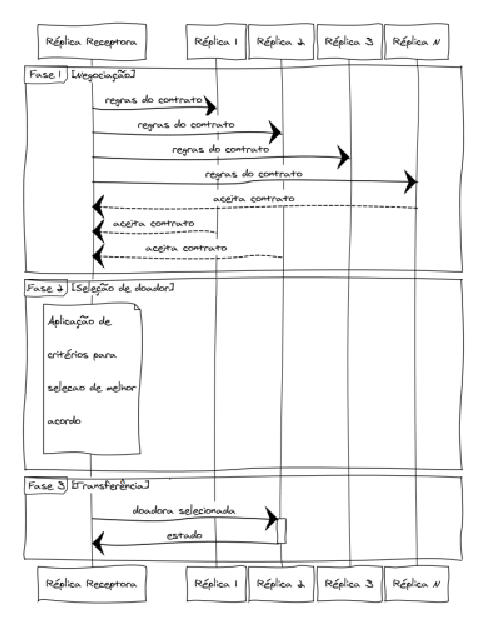
\includegraphics[width=11cm]{conteudo/capitulos/figuras/fases_protocolo.eps}
  \caption{Fases do protocolo de transferência de estado}
  \label{fig:fases_protocolo}
\end{figure}

Na Fase de Negociação, fase inicial, a réplica receptora estabelece as regras da
transferência de estado através da mensagem \classname{PolicyMessage}. Por exemplo,
supomos que, independente do motivo, uma réplica $r$ deseje receber um estado a partir da
instância de consenso $240$. Então, $r$ inicia a negociação de estado difundindo a
mensagem contratual. As réplicas que recebem essa mensagem de solicitação de negociação de
estado são solidárias e tentam atender essa requisição. Elas avaliam as exigências
contidas na mensagem e, caso estejam de acordo, enviam, somente para a replica receptora
(remetente do contrato), a mensagem \classname{DealMessage}. Essa proposta acordo, contém
informações referentes ao estado que a réplica doadora está oferecendo.

Caso a réplica receptora não receba nenhuma proposta de acordo após um tempo
pré-estabelecido, ela reinicia a Fase de Negociação até encontrar uma réplica doadora.
Podemos nos beneficiar desse \emph{loop} inicial que se encontra a réplica receptora para
criarmos diferentes políticas contratuais para transferência de estado. Nessa versão
proposta de Treplica, supomos configurações de duas politicas: uma mais agressiva e outra
mais ingênua. Lembrando que todas as políticas devem fornecer qual é a instância de
consenso pretendida.

\begin{itemize}
  \item Somente réplicas leitoras: essa política é mais restritiva, busca um acordo com
    uma réplica leitora \footnote{Réplicas leitoras são aquelas onde apenas os agentes
    proponente e aprendiz estão em execução. Elas não assumem um papel fundamental na
    execução de Paxos. Trataremos réplicas leitoras na \autoref{sec:replicas_leitoras}}.
    Acordos com réplica leitoras são preferíveis devido à restrição de sincronia exigida
    pelo protocolo. Dessa forma, essa política tenta minimizar possíveis impactos na
    computação de Paxos.
  \item Qualquer réplica: essa política é a menos restritiva possível, busca um acordo
    independente da configuração da réplica.
\end{itemize}

Devemos ter cuidado ao eleger uma réplica votante como réplica doadora, pois podemos gerar
impacto direto no desempenho da aplicação. A réplica doadora não participará da eleição de
um novo estado durante o período que está transmitindo seu estado (congelamento do estado
para garantia de consistência). Lembrando que, no algoritmo Paxos, a partir do momento em
que a maioria dos receptores concordam com a alteração do estado, mais cedo ou mais tarde
todas as réplicas chegarão ao mesmo estado. A partir do momento que retiramos
temporariamente da computação uma réplica votante, a probabilidade de atingir consenso
pela maioria diminui, podendo até impossibilitar o progresso do algoritmo.

O protocolo progride quando a réplica receptora possui propostas de acordo. Quando essa
condição é alcançada, ela inicia a Fase de Seleção de Doadora. Fase que executa um
algoritmo simples capaz de eleger a réplica que propôs o melhor acordo. Somente a partir
do momento que o algoritmo estabelece uma réplica doadora a Fase de Transferência inicia.
Para a execução dessa fase, os seguintes aspectos de Treplica foram considerados: (1) o
estado de uma aplicação pode ser tão grande quanto a capacidade de memória de uma réplica;
(2) todas as mensagens são trocadas utilizando o protocolo UDP.

Optamos então pela utilização do protocolo TCP para transferência de estado cobiçando
maior vazão dos dados nessa operação \cite{abdellatif04}. Somente o estado é enviado via
TCP, todas as outras mensagens pertencentes ao protocolo utilizam comunicação UDP, nativa
de Treplica. Sendo assim, a réplica receptora abre um \emph{socket} TCP e envia a mensagem
\classname{GETMessage} para a réplica doadora com o endereço do \emph{socket} TCP
recentemente aberto. Por sua vez, a réplica doadora bloqueia suas atividades e estabelece
a conexão TCP com a réplica leitora. Finalmente a transferência de estado é executada.

Assim que a operação é concluída, a conexão TCP entre as réplicas é finalizada. A réplica
doadora volta para computação e a réplica leitora começa a processar as requisições
encaminhadas pelos seus clientes. Estabelecemos um \emph{timeout} para evitar bloqueios
indevidos por falha em alguma das réplicas envolvidas na transação. Caso todas as etapas
do protocolo não sejam concluídas em no máximo 10 segundos, a negociação de estado é
reiniciada até que se obtenha êxito. A \autoref{fig:protocolo} ilustra o funcionamento do
protocolo com suas respectivas trocas de mensagens.

\begin{figure}[ht]
  \centering
  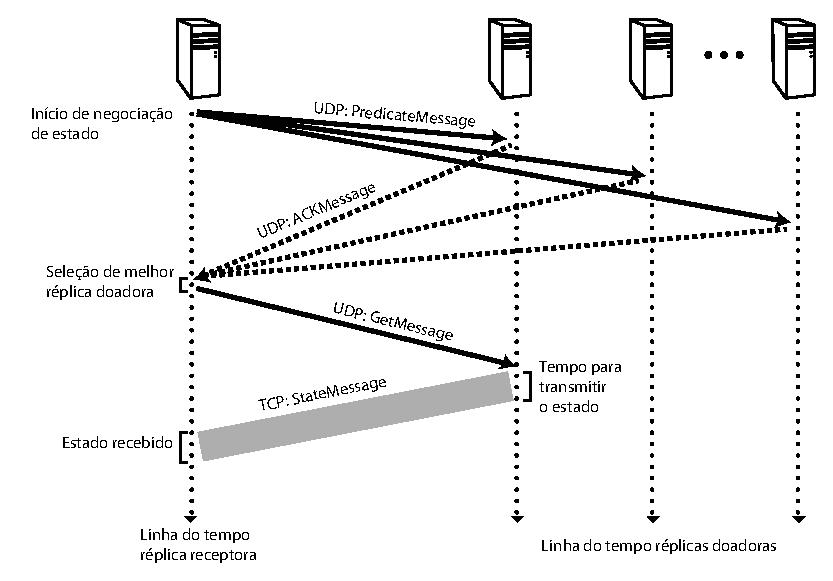
\includegraphics[width=11cm]{conteudo/capitulos/figuras/transferencia_estado.eps}
  \caption{Protocolo de transferência de estado}
  \label{fig:protocolo}
\end{figure}

\subsubsection{Componentes alterados}

O protocolo de transferência de estados possui quatro mensagens que são representadas
pelas classes \classname{PolicyMessage}, \classname{DealMessage}, \classname{GetMessage} e
\classname{StateMessage}. Todas essas classes implementam a interface de marcação
\classname{StateTransferMessage}, possibilitando assim, distinguir as mensagens do
protocolo das mensagens de Paxos.

Todas as mensagens do protocolo são roteadas no \emph{main loop} de cada réplica para a
classe \classname{Diplomat}, responsável pelo tratamento dessas mensagens, independente da
configuração existente na réplica.

\subsubsubsection{PolicyMessage}

A classe \classname{PolicyMessage} é a primeira mensagem do protocolo para transferência
de estado. Essa classe além de sinalizar para as outras réplicas do grupo que existe uma
réplica interessada em receber um estado, contém todas as informações sobre o estado
pretendido pela réplica receptora.

Os dados contratuais são abstraídos pela classe \classname{Policy}. Essa classe por sua
vez, contém o número da instância de consenso desejado (informação mínima para proposta de
um acordo) e uma lista de regras qualificadoras, que uma réplica deve atender para ser uma
doadora.

\subsubsubsection{DealMessage}

A classe \classname{DealMessage} também pertence ao grupo de mensagens trocadas pelo
protocolo de transferência. Essa classe abstrai uma proposta de acordo. Ela é uma
sinalização para a réplica receptora, informa a existência de uma réplica disposta a dor
seu estado (réplica doadora está em conformidade com a política estabelecida pela réplica
receptora). Quanto mais mensagens propondo acordo de transferência uma réplica receptora
receber, menos restritivas são suas políticas, potencializando a seleção de uma réplica
votante.

\subsubsubsection{GetMessage}

A classe \classname{GetMessage} é a abstração da mensagem de pedido de estado enviada
somente para a réplica doadora. As informações do endereço para envio do estado (através
de \emph{socket} TCP) é extraído dessa mensagem.

\subsubsubsection{StateMessage}

A classe \classname{StateMessage} é a abstração do estado enviado da réplica doadora para
a réplica receptora. Essa classe possuí como atributos o número da instância de consenso
(último decreto que causou alteração no estado) e um estado no formato
\classname{java.io.Serializable}. Definimos essa classe como uma cópia instantânea, tirada
no no período que a réplica está bloqueada para alterações.

A partir do conteúdo armazenado por \classname{StateMessage}, qualquer réplica que possuí
uma visão de estado menor \footnote{Podemos supor comparações de estados através da última
instância de consenso, já que o mesmo é um limiar crescente \cite{vieira-10b}.} pode se
beneficiar da substituição de seu estado local corrente (desatualizado) por um mais atual,
com potencial chance de ser o estado corrente compartilhado pela maioria grupo, conforme
especificação de Paxos.

\subsubsubsection{Diplomat}

A classe \classname{Diplomat} é responsável por implementar o tratamento das mensagens do
protocolo de trasferência. Toda réplica, independente da configuração, possui uma
instância da classe \classname{Diplomat} para representar seus interesses frente outras
réplicas. A abstração desse componente foi inspirada nas funções de diplomacia (ciência e
arte referentes às relações entre Estados \cite{aurelio}) exercidas por um Diplomata no
modelo atual de relação entre nações \footnote{Segundo \citeonline{aurelio}, diplomata é
um funcionário que representa um governo junto de outro governo.}.

O Diplomata adéqua suas funções de trabalho conforme o estado corrente da replica. Em uma
réplica receptora, está habilitado as funções responsáveis por obter um novo estado:
criação de política, seleção de réplica doadora e abertura de \emph{socket} TCP. Por outro
lado, em uma réplica doadora as funções para ceder o estado é que estão habilitadas:
análise de aderência a política de transferência, bloqueio de alterações de estado e o
envio de estado.

Para seleção da melhor proposta de transferência de estado, o Diplomata armazena em
memória todas as propostas recebidas e após o estouro de um \emph{timeout} estabelecido, a
seleção é realizada. Consideramos como melhor proposta de estado aquela que possui maior
instância de consenso. Em caso de eventuais erros e/ou \emph{timeouts} as propostas são
removidas da memória para evitar conflitos com as futuras propostas de acordo, que serão
recebidas devido atuação do mecanismo de reinicialização.

\subsubsection{Política de Reconfiguração}

Identificamos dois potenciais pontos que se beneficiariam da utilização do protocolo de
transferência de estado: (1) expansão do aglomerado e (2) recuperação de erros. Para a
construção desse trabalho, focamos na aplicação do protocolo na expansão do aglomerado,
conforme ilustra a \autoref{fig:inclusao}. Supomos alguns aspecto para serem considerados:

\begin{itemize}
  \item O estado da nova réplica que deseja se juntar ao aglomerado está defasado com
    relação ao estado das réplicas que já participam do grupo. É imprescindível que essa
    defasagem seja suprimida.
  \item A operação para igualar o estado da nova réplica com o estado compartilhado pelo
    grupo deve ser consistente.
  \item O impacto gerado para o processamento do aglomerado deve ser mínimo.
\end{itemize}

Para justificar a inclusão de uma nova réplica, obrigatoriamente é preciso geração de
benefícios para o processamento em grupo, caso contrário estamos executando operações sem
serventia com potencial para saturar o sistema.

\begin{figure}[ht]
  \centering
  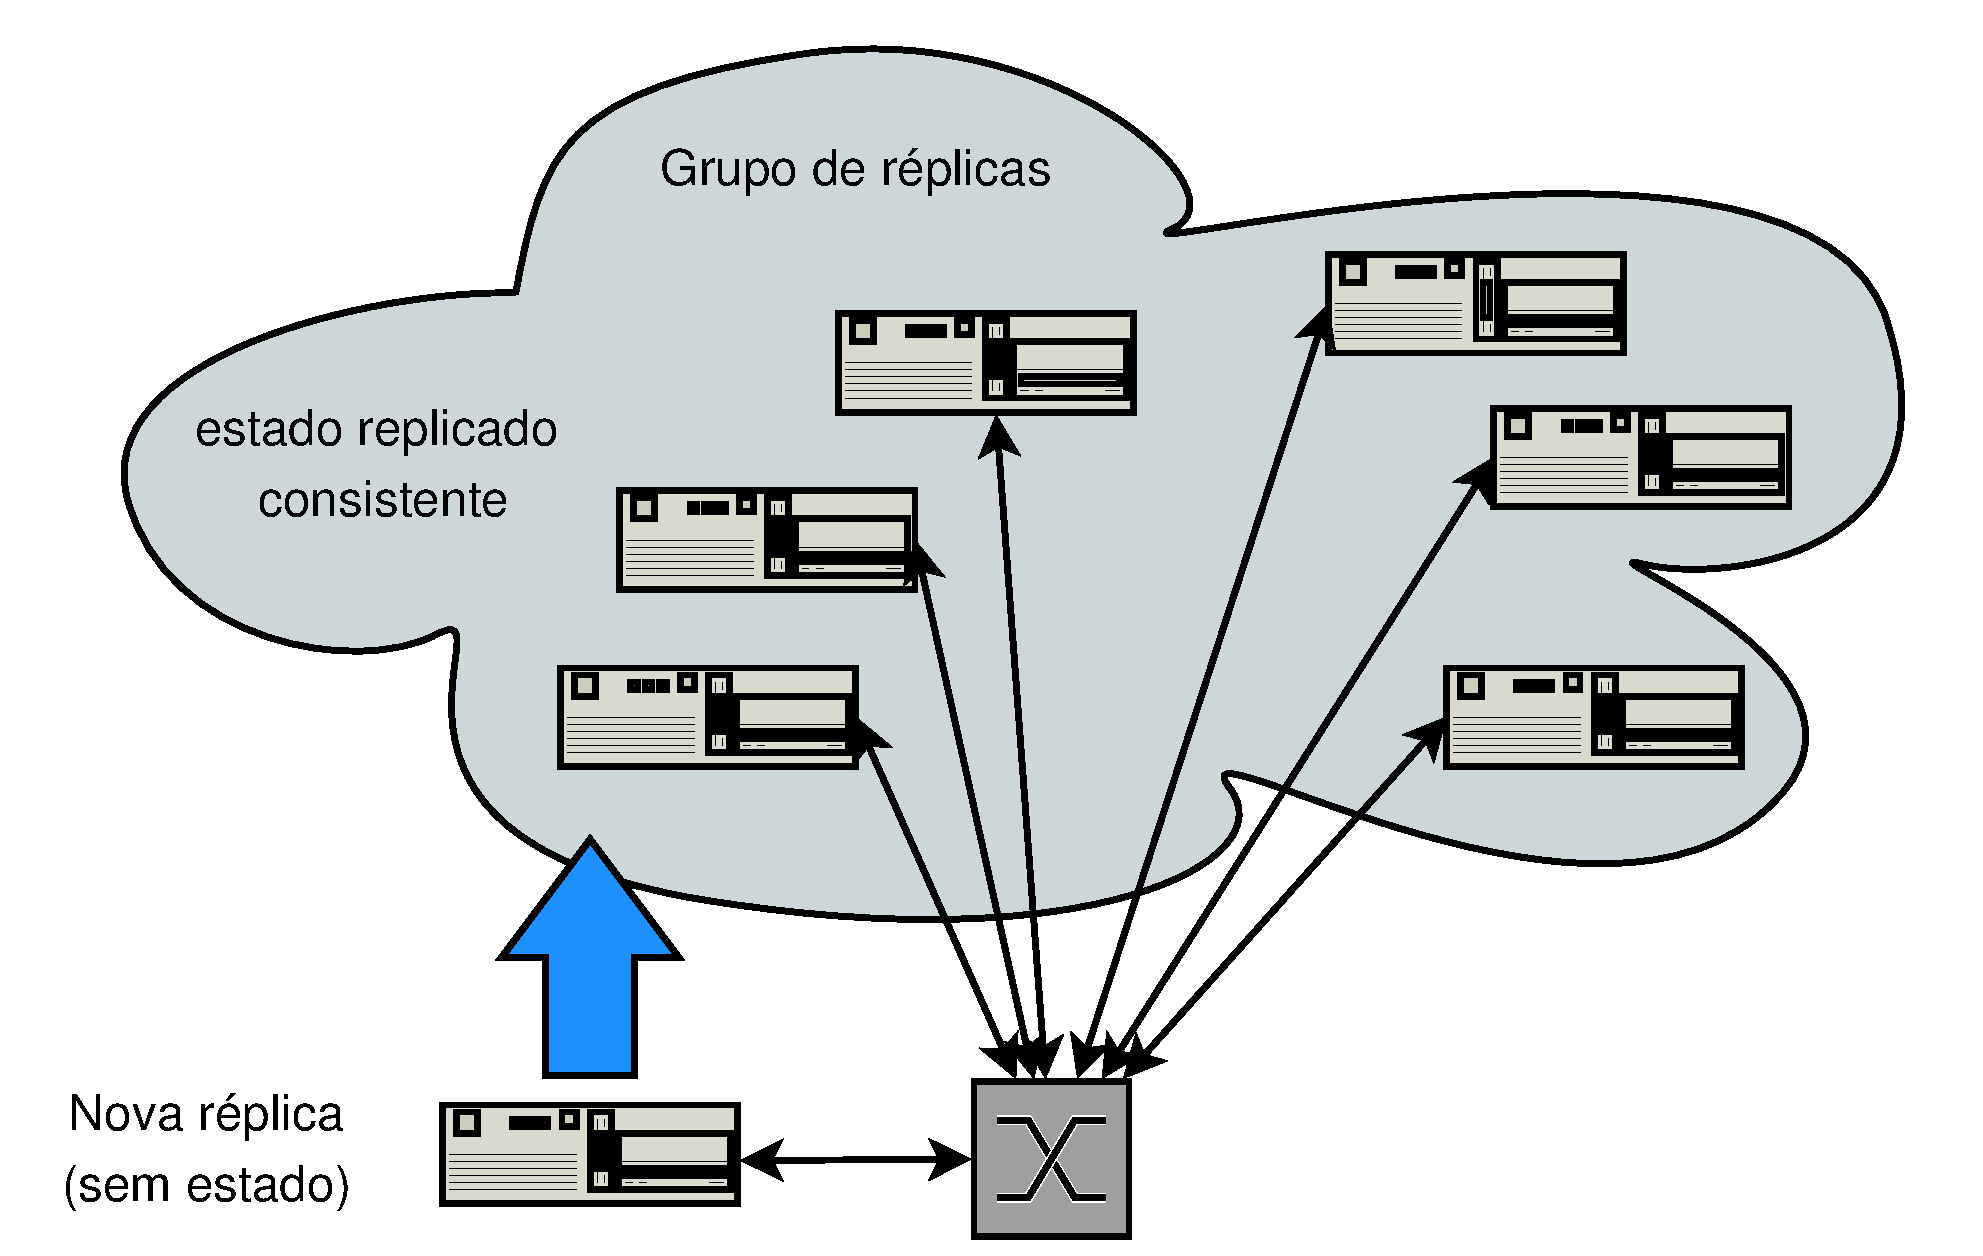
\includegraphics[width=11cm]{conteudo/capitulos/figuras/inclusao_replica_cluster.eps}
  \caption{Inclusão de réplica}
  \label{fig:inclusao}
\end{figure}

\citeonline{lamport10} apresenta em seu trabalho um mecanismo para reconfiguração que pode
ser aplicados em réplicas votantes, através da criação de diferentes formações de grupos
representados por visões, controladas por um identificador sequencial. Como estamos
trabalhando no modelo computacional assíncrono com falha-e-recuperação, a aplicação dessa
proposta é complexa. Se analisarmos um instante no tempo, diferentes visões poderão estar
sendo executadas simultaneamente com a visão corrente (visão com maior identificador). O
gerenciamento dessas visões e a formação de diferentes grupos não é uma tarefa trivial.

Investimos nosso esforço na construção de um mecanismo que tenta fugir da complexidade do
mecanismo de visões proposto por \citeonline{lamport10}, consequentemente evitamos
reconfigurações em réplicas votantes e focamos na criação e remoção de réplicas leitoras.
A motivação por trás da criação de réplicas leitoras é permitir que o sistema reaja de
forma autônoma a picos de carga sem comprometer o desempenho do mesmo. No entanto, sem uma
política cuidadosa de reconfiguração corre-se o risco de gastar muitos dos recursos do
sistema no próprio processo de reconfiguração, anulando quaisquer ganhos advindos do
acréscimo de novas réplicas leitoras.

A política de reconfiguração deve, desta forma, ser um equilíbrio entre o custo de se
instanciar uma nova réplica leitora e os ganhos de desempenho a serem auferidos após esta
instanciação. O trabalho de especificação de parâmetros para esta política ainda está em
seu estágio inicial, dependendo de estudos mais aprofundados para caracterizar os custos
envolvidos.

\subsection{Paxos com Réplicas Leitoras}\label{sec:replicas_leitoras}

A ideia principal da abordagem proposta é utilizar réplicas que não participem do processo
de decisão de instâncias de consenso. Isso é feito com a adoção de \emph{réplicas
leitoras}, que são réplicas onde apenas parte dos agentes do algoritmo Paxos estão
executando. Para maior clareza de exposição, quando necessário, chamaremos as réplicas
contendo todos os agentes ativos de \emph{réplicas votantes}. Para suportar a adaptação
elástica a novos perfis de desempenho, desenvolvemos um mecanismo para o
\emph{provisionamento de réplicas} e uma \emph{política de reconfiguração}.

\subsubsection{Réplicas Leitoras}

Réplicas leitoras são réplicas onde apenas os agentes proponente e aprendiz estão
executando. Dessa forma, do ponto de vista do conjunto de processos que implementam o
algoritmo Paxos, uma réplica leitora é capaz apenas de propor operações a serem aplicadas
no estado replicado e de aprender operações decididas pelo conjunto de receptores. Do
ponto de vista do cliente da aplicação replicada um réplica leitora se comporta como uma
réplica votante: ela atende requisições de qualquer tipo garantindo a execução atômica das
mesmas.

As réplicas leitoras não assumem um papel fundamental na execução do algoritmo Paxos, no
entanto elas se integram de forma consistente com a operação das réplicas votantes por
meio de suas funções fundamentais: propor e aprender requisições de escrita. As réplicas
leitoras propõem novas requisições a serem executadas em nome de seus clientes através de
seu agente proponente. O proponente encaminha a operação ao coordenador que por sua vez
decide, em conjunto com os receptores, a ordem da mesma através de uma rodada de Paxos,
como descrito no \autoref{cap1:replicacao_ativa_paxos}. Uma vez que a decisão é alcançada,
a mesma é difundida para o resto do sistema. Nesse momento o agente aprendiz da réplica
leitora toma conhecimento da decisão e atualiza o seu estado interno, sem a participação
ativa do coordenador ou de qualquer receptor.

Tanto o processo de proposta quanto o de aprendizado executado por uma réplica leitora
devem usar as mesmas estratégias de implementação das réplicas votantes. Na verdade, em
nossa implementação usando Treplica, as réplicas leitoras foram construídas a partir da
separação modular dos agentes que implementam Paxos. Dessa forma, reutilizamos os mesmos
componentes e por consequência essas réplicas são capazes de detectar e reenviar propostas
perdidas, detectar e corrigir lacunas na sequência de instâncias de consenso, fazer
controle de fluxo e de congestionamento, entre outras operações fundamentais para uma
operação eficiente de Paxos \cite{vieira-tr10b}.

Uma consequência importante do uso de réplicas leitoras é que essas réplicas,
consistentemente com as funções que elas assumem no algoritmo Paxos, não precisam de
memória persistente para sua operação. Isso se deve ao fato de que elas não executam as
Fases 1 e 2 do algoritmo. Porém, pode ser interessante que essas réplicas registrem a
proposta decidida de forma a não precisar realizar uma recuperação completa em caso de
falha. Na nossa proposta de réplicas leitoras decidimos não fazer esse registro de forma a
remover completamente a escrita em memória persistente do caminho crítico de execução. É
interessante observar que a escrita eliminada ocorre somente quando a réplica leitora
atualiza o seu estado de acordo com as propostas decididas pelos receptores das réplicas
votantes. Dessa forma, as réplicas leitoras conseguem manter seu estado atualizado com as
réplicas votantes com um custo mínimo. Elas também são capazes de processar requisições de
escrita com um custo similar àquele gerado pelas réplicas votantes ao executar as mesmas
requisições. Podemos argumentar que esse custo é menor, na medida que as réplicas leitoras
aliviam as réplicas votantes do custo de manter as conexões abertas com os clientes.

Utilizando réplicas leitoras, podemos formar grupos de réplicas com diferentes graus de
uso de memória persistente \cite{aguilera00}. Uma configuração simples seria mesclar
réplicas votantes e leitoras formando um conjunto híbrido de réplicas transparente para o
cliente, conforme ilustra a \autoref{fig:configuracao_replicas_leitoras} (a). É concebível
ainda uma configuração onde as réplicas votantes não entram em contato com os clientes,
sendo essa operação completamente delegada às replicas leitoras, configuração ilustrada
pela \autoref{fig:configuracao_replicas_leitoras} (b).

\begin{figure}[ht]
  \begin{center}
    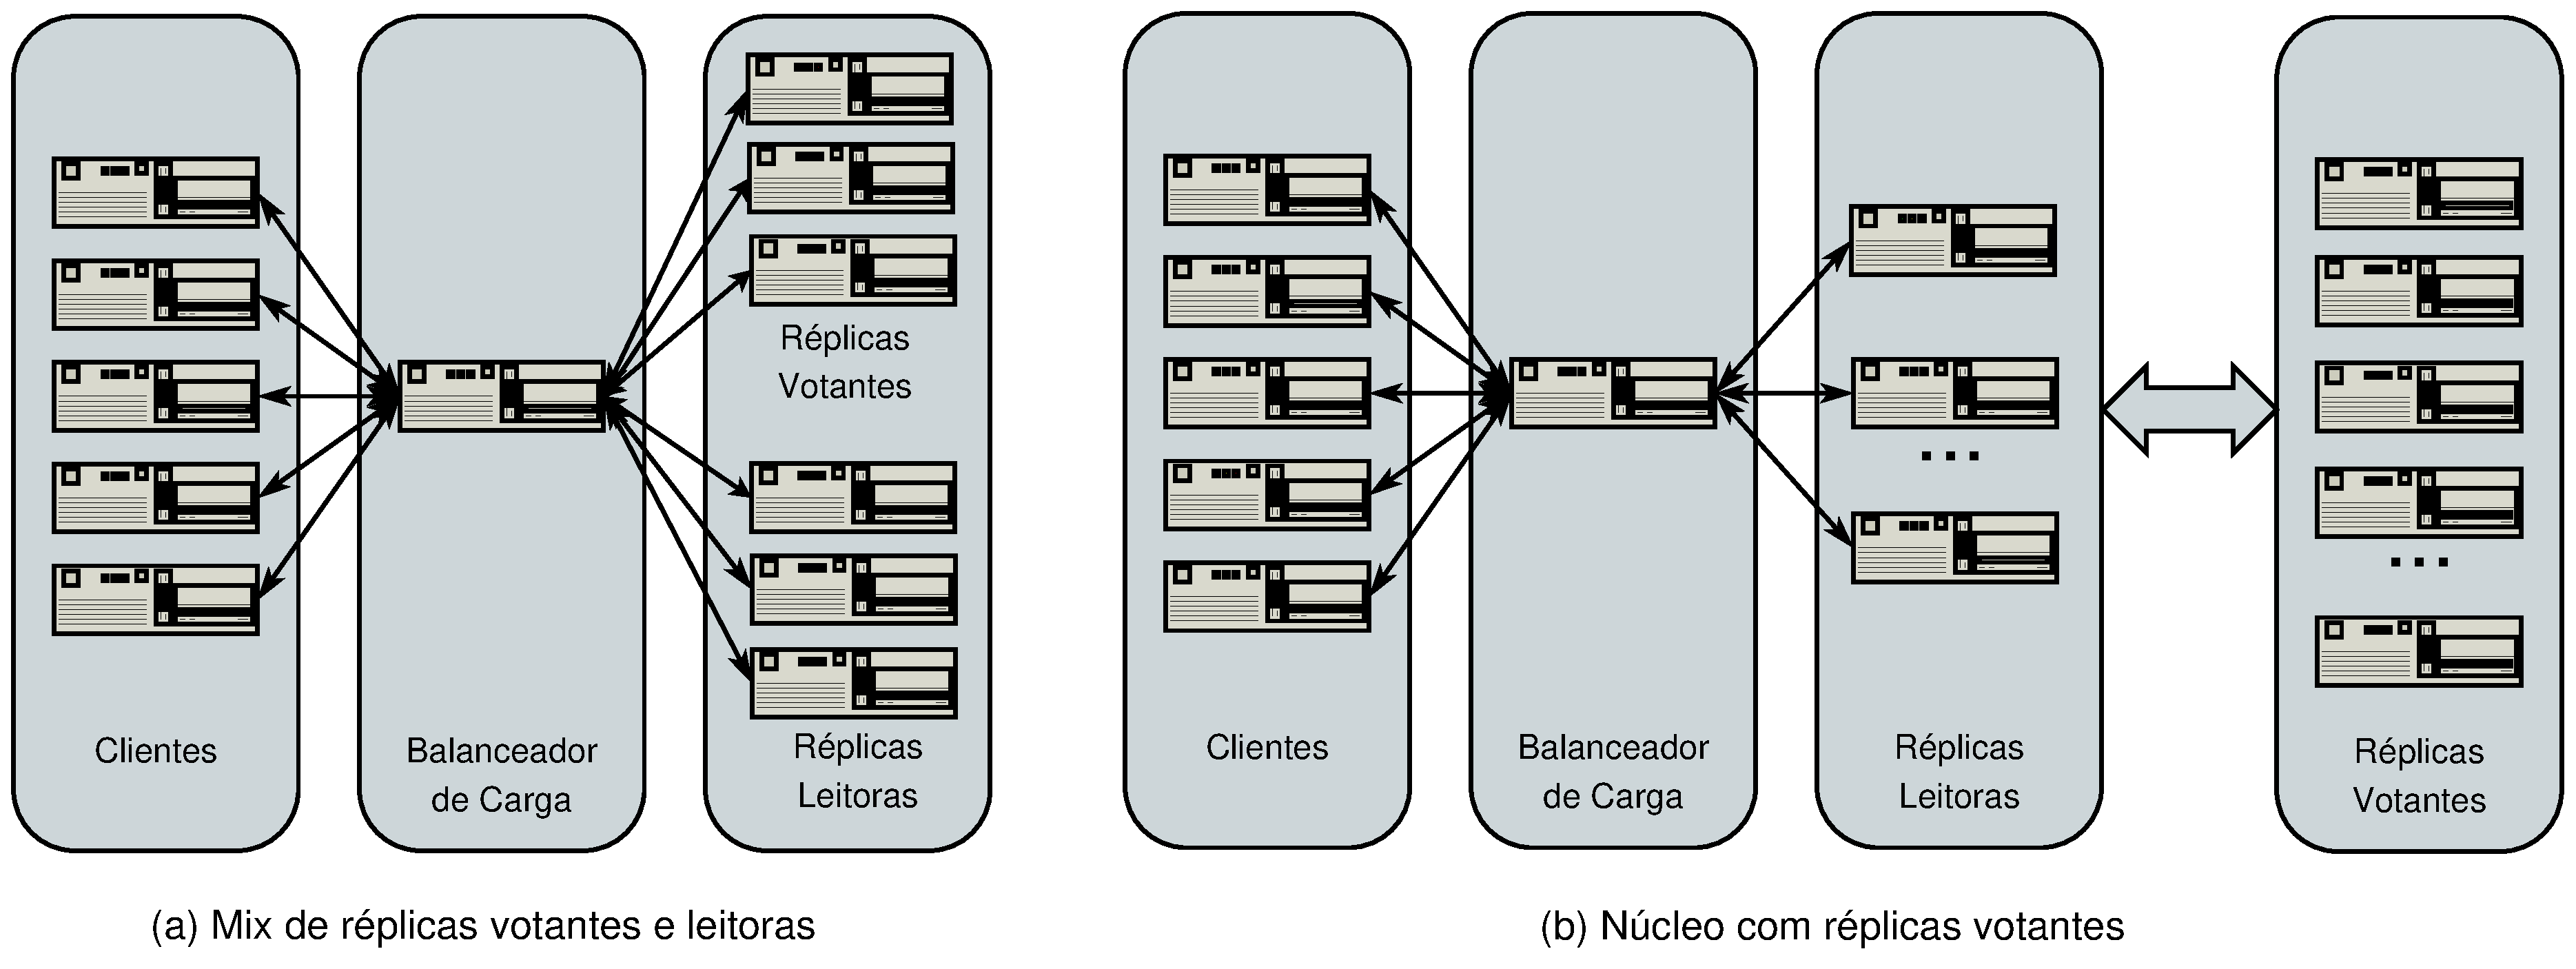
\includegraphics[width=16cm]{conteudo/capitulos/figuras/configuracao_replicas_leitoras.eps}
  \end{center}
  \caption{Configuração de Paxos com réplicas votantes e leitoras}
  \label{fig:configuracao_replicas_leitoras}
\end{figure}

As réplicas leitoras funcionam então como uma espécie de cache \emph{write-through}
distribuído. O estado replicado na memória destas réplicas permite atender diretamente as
requisições de leitura dos clientes, enquanto as requisições de escrita são repassadas ao
receptores. Podemos ver claramente que a taxa de acerto desse cache está diretamente
ligada à proporção de operações de leitura geradas pelos clientes e que a vazão de
operações de leitura tem o potencial de crescer linearmente com o número de réplicas
leitoras disponíveis.

\subsubsection{Componentes alterados}

Antes de detalharmos as alterações realizadas, vamos recapitular de forma resumida a
iteração entre os agentes de Paxos: proponentes enviam a sua proposta para o coordenador
que tenta alcançar consenso sobre a proposta em uma rodada, sendo que cada proposta
corresponde a uma ou mais requisições de escrita da aplicação sendo replicada.

Anteriormente, era possível uma única configuração de réplicas que empregava todos os
agentes de Paxos utilizando memória persistente. A nova funcionalidade de réplicas
leitoras foi implementada através de uma segregação modular dos agentes utilizados por uma
réplica votante:

\begin{itemize}
  \item Proponente: agente capaz de propor valores;
  \item Receptor: agente que vota em uma única proposta por rodada;
  \item Aprendiz: agente que aprende a decisão de consenso;
  \item Coordenador: agente responsável por garantir o funcionamento do algoritmo a cada
    rodada de consenso executada.
\end{itemize}

A classe denominada \classname{PaxosPersistentQueue} é responsável por implementar o
agrupamento de todos esses agentes, caracterizando assim uma réplica votante. Podemos
definir, do ponto de vista de uma Máquina Virtual Java (JVM), que uam réplica votante
possui como uma das suas \emph{threads} ativas o \emph{main loop} da classe
\classname{PaxosPersistentQueue}. Em contra partida, uma réplica leitora, executa o
\emph{main loop} da classe \classname{PaxosReadonlyQueue}. Essa classe, implementa somente
a agregação dos agentes proponente e aprendiz, sem a utilização de memória persistente.
Detalharemos nas próximas seções a implementação proposta para esse componente.

\subsubsubsection{PaxosReadonlyQueue}

A classe \classname{PaxosReadonlyQueue} foi criada para fornecer o mesmo comportamento da
classe \classname{PaxosPersistenteQueue}: disponibilizar uma fila que será utilizada pelo
protocolo Paxos. No entanto, as operações suportadas por \classname{PaxosReadonlyQueue}
não as mesmas. Do ponto de vista do processamento de mensagens postadas na fila, as
seguintes propriedades foram supostas para caracterizar uma réplica leitora:

\begin{itemize}
  \item Abdicar liderança: todas as mensagens relacionadas a eleição de líder não são
    processadas, logo é eliminada qualquer possibilidade de uma réplica leitora se tornar
    coordenadora de uma rodada de Paxos.
  \item Inelegível ao voto: mensagens relacionadas a votação de uma proposta são
    ignoradas. Dessa forma, réplicas leitoras não participam do processo de decisão de
    consenso e não são essenciais para o progresso do algoritmo Paxos.
  \item Aprendizado: todas as mensagens endereçadas ao componente \classname{Learner} são
    processadas pela fila. Consequentemente, os mecanismos descobrir qual foi o consenso
    de uma determinada rodada são habilitados.
\end{itemize}

O principal objetivo dessa classe é participar das operações que não exigem dados
persistentes para garantir correção do algoritmo, oferecendo instâncias capazes de atuar
parcialmente nas fases de Paxos. Do ponto de vista do cliente da aplicação um réplica
leitora se comporta como uma réplica votante: ela atende requisições de qualquer tipo
garantindo a execução atômica das mesmas. Sendo assim, as seguintes premissas não podem
ser violadas:

\begin{itemize}
  \item Mensagens quem alteram o estado (escrita): são resolvidas pelo aglomerado de
    réplicas orquestrado pelo protocolo Paxos, porém réplicas que não possuem grau de
    memória persistente não participam da decisão de consenso.
  \item Mensagens que não alteram estado (leitura): são resolvidas localmente independente
    do grau de memória da réplica.
\end{itemize}

Do ponto de vista de uma réplica votante, não é possível distinguir se a proposta é
oriunda de uma réplica votante ou leitora. O mecanismo para configuração do grau de
memória de uma réplica em Treplica atua de forma transparente junto com protocolo Paxos,
respeitando a forte premissa: o número de réplicas leitoras nunca deve afetar o número de
réplicas votantes. Sendo assim, podemos afirmar que o progresso e a correção do algoritmo
não são violados.

Réplicas oferecem um poder de manobra para aliviar a carga de processamento das réplicas
votantes com relação a mensagens de leituras, podendo ser configuradas de tal forma que
nenhuma mensagem de leitura seja processada por uma réplica votante. Avaliar e propor
soluções para configuração do conjunto de réplicas não faz parte do escopo desse trabalho.

\subsubsubsection{WeakSecretary}

A classe \classname{WeakSecretary} apresenta uma abstração de I/O sem persistência de
dados em disco. Esse componente é uma versão leve da classe \classname{Secretary}
(\autoref{subsec:secretary}), ela é utilizada pelos agentes de Paxos para enviar mensagens
pela rede, através do intermédio do componente \classname{Transport}
(\autoref{subsec:transport}). Essa classe foi projetada para trabalhar com dados somente
em memória, dessa forma todos os dados computados são perdidos na presença de defeitos na
réplica. No entanto, na ausência de falhas nos beneficiamos da eliminação de uma operação
custosa relacionada com I/O em disco.

\classname{WeakSecretary} também é responsável por lidar com o componente
\classname{Ledger} (\autoref{subsec:ledger}) e com a fila de objetos utilizada
para entregar mensagens para a camada da aplicação. A principal razão para a criação dessa
abstração em Treplica foi eliminar a operação de persistência em disco, gerando um
componente volátil, capaz de oferecer as operações essenciais para o progresso do
algoritmo sem o ônus da escrita em disco.

\subsubsection{Provisionamento de Réplicas Leitoras}

É possível utilizar os mecanismos tradicionais de Treplica para provisionar uma nova
réplica leitora. Em resumo, uma réplica que se integra ao sistema pela primeira vez ou
após uma falha demorada deve recuperar o seu estado. Esse processo acontece através de um
mecanismo de preenchimento de lacunas, que observa que não pode executar novas requisições
de escrita sem antes executar as requisições anteriores \cite{vieira-tr10b}. Esse
procedimento é voltado para reparar pequenas interrupções e não a recuperação do estado
completo de uma réplica. Em particular, no caso de uma réplica leitora sem estado
persistente, o tamanho dessa recuperação pode ser muito grande em termos do número de
\emph{requisições} a serem reexecutadas, pois ela sempre parte do estado inicial vazio.

Foi necessário então criar um procedimento de provisionamento de réplicas, de forma a
permitir o rápido início de uma réplica leitora. Esse mecanismo não é necessariamente
exclusivo de réplicas leitoras e pode ser aplicado a réplicas normais. Porém, neste
primeiro momento, ele tira proveito do fato dessas réplicas não terem memória persistente.
Em particular, a adição ou remoção de uma réplica leitora não altera o número de
receptores executando o algoritmo, não havendo necessidade de se realizar um
reconfiguração custosa \cite{lamport10}.

\subsection{Transferência de estado para recuperação de falhas}

Treplica possui outro potencial candidato para empregar o protocolo de transferência: o
componente detector lacunas na sequência de instâncias de consenso. Lacunas podem surgir
por diferentes motivos: falha-e-recuperação na réplica, perda de mensagens ou ainda
réplicas com grandes diferenças de capacidade de processamento. Para preencher lacunas
detectadas, o componente solicita retransmissão da instância de consenso em uma
determinada rodada. É perceptível que na presença de grandes lacunas essa abordagem
exigirá uma longa sequência de retransmissões.

Para exemplificar o potencial problema do detector de lacunas, vamos supor que a aplicação
$x$ está passando por um grande pico de processamento (\emph{flash crowds}) e que a
réplica $r$ possui uma grande lacuna. O mecanismo detector de lacunas solicitará
retransmissão das instâncias de consenso não conhecidas por ele, aumentando a concorrência
no meio compartilhado pelas réplicas: a rede. Como solução alternativa, podemos utilizar o
mecanismo de transferência, para concentrar em uma única mensagem, o estado resultante das
aplicações das instâncias de consenso. Dessa forma, o novo mecanismo suposto para detectar
lacunas tem capacidade de:

\begin{itemize}
  \item Retransmissão de instância de consenso: utilizado para preencher pequenas lacunas
    na sequência de consenso.
  \item Protocolo de transferência de estado: utilizado para preencher grandes lacunas,
    onde retransmissão tem potencial perda de desempenho.
\end{itemize}


\chapter{Avaliação e Resultados}\label{cap3}

O \autoref{cap1:treplica_reconfiguravel} apresentou três funcionalidades para expansão da
biblioteca Treplica:

\begin{enumerate}
  \item Protocolo para transferência de estado: criação de um mecanismo eficiente para
    transferência de estado entre réplicas.
  \item Réplicas leitoras: possibilidade da utilização de réplicas que não participam do
    processo de decisão de instâncias de consenso.
  \item Equalização de estado: proposta para novo componente de preenchimento de lacunas
    originadas por possíveis períodos de instabilidade da réplica e/ou falhas.
\end{enumerate}

Supomos duas hipóteses baseado-se nas alterações propostas 1 e 2. A alteração proposta
pelo item 3 não será validada por esse trabalho. Mantivemos a descrição dessa alteração
para enriquecimento do conteúdo e possível utilização em trabalhos futuros.

\begin{enumerate}
  \item Se possuirmos um mecanismo transferência eficiente, podemos recuperar o estado de
    uma réplica de forma mais eficiente que a aplicação do histórico de decreto do
    aglomerado. Lembrando que, toda réplica votante armazena em memória persistente
    qualquer alteração realizada no seu estado.
  \item Se possuirmos uma réplica que evite a reconfiguração total do sistema, ganharemos
    o poder de manobra necessário para expansão do aglomerado de acordo com a demanda de
    clientes.
\end{enumerate}

Para validar que a hipótese 1 e 2 podem aumentar o desempenho de um sistema que utiliza a
biblioteca Treplica, supomos uma carga de trabalho na qual uma parcela significativa das
requisições solicitadas para aplicação seja de leitura. Essa é uma suposição razoável para
a maioria das aplicações de Internet \cite{tpc02} e proporciona o cenário, que acreditamos
ser o mais adequado, para execução eficiente utilizando réplicas leitoras.

Começamos esse capítulo com a \autoref{sec:aplicacao}, apresentando os detalhes da
aplicação e as bibliotecas utilizadas para sua concepção. Em seguida, na
\autoref{sec:ambiente_experimental} descrevemos o ambiente experimental usado na execução
dos experimentos. As próximas duas seções \autoref{sec:experimento_tranferencia_extado} e
\autoref{sec:experimento_replicas_leitoras} apresentam respectivamente os experimentos de
transferência de estado e réplicas leitoras com seus respectivos cenários, resultados e
análise. Encerramos o capitulo com a \autoref{sec:trabalhos-relacionados} apresentando as
considerações finais.


\section{Aplicação}\label{aplicacao}

Para fins experimentais, desenvolvemos então, visando a validação do conjunto de
experimentos, uma aplicação Web simples que mapeia uma cadeia de caracteres para um valor
numérico de 32 bits. Em outras palavras, criamos uma aplicação caracterizada como um mapa
que disponibiliza dois serviços aos clientes remotos através de uma interface HTTP:

\begin{enumerate}
  \item Operação GET \cod{/replicated-map/map/key/<chave>}
  \item Operação PUT \cod{/replicated-map/map/key/<chave>/value/<valor>}
\end{enumerate}

A operação GET é uma operação de leitura, sua função proporciona ao cliente buscar o valor
armazenado em uma determinada chave. Definimos que uma operação bem-sucedida no método GET
retorna o código de status HTTP 200 e um JSON com o valor da chave requisitada
\verb|{"value":"<valor>"}|. Por outro lado, o método PUT defini operações de escrita, ele
é responsável por armazenar um valor em uma determinada chave. Definimos que uma operação
de escrita sem falhas não possui corpo de retorno, o método retorna apenas o código de
status HTTP 201.

Utilizamos a linguagem Scala\footnote{http://www.scala-lang.org} para criação da
aplicação, sendo que o estado da aplicação é gerenciado pela biblioteca Treplica que atua
como um \emph{middleware} de replicação ativa, conforme ilustra a figura
\autoref{fig:treplica_como_middleware}. Treplica é uma biblioteca Java e mostrou boa
interoperabilidade com a aplicação. Não relatamos nenhum problema oriundo da utilização de
bibliotecas Java com a linguagem Scala.

\begin{figure}[ht]
  \centering
  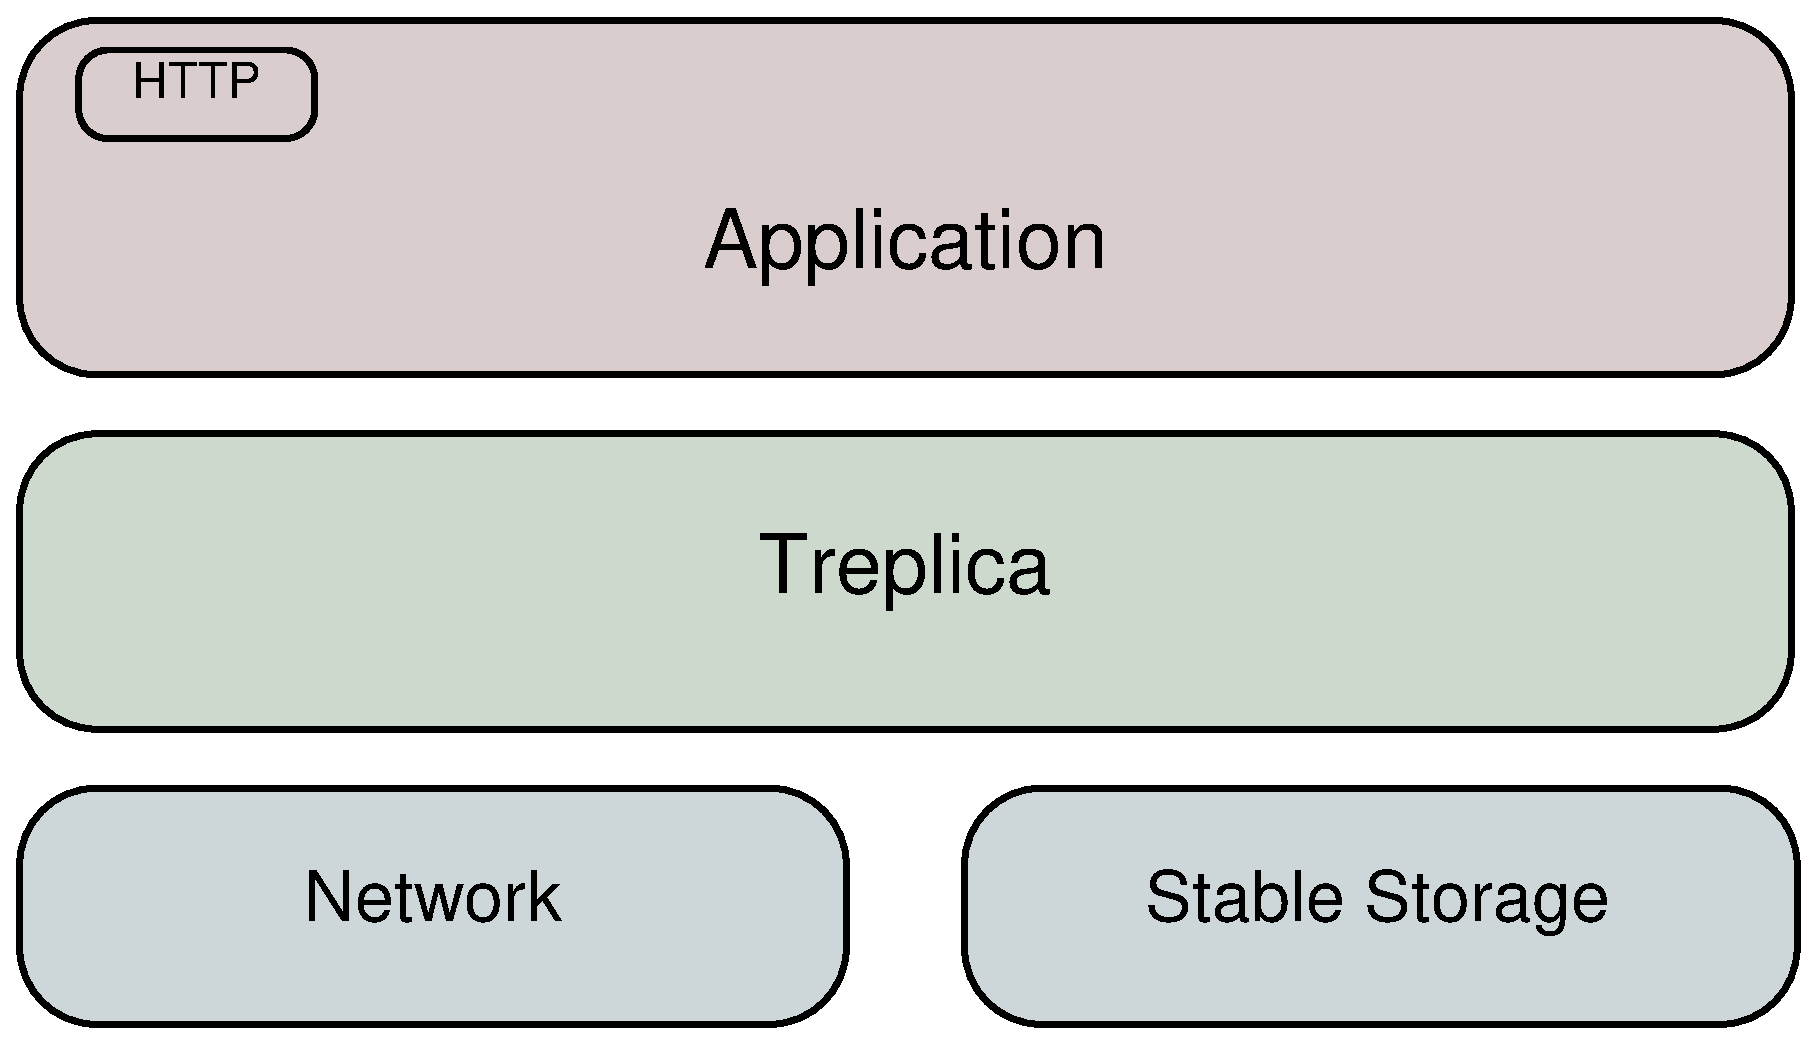
\includegraphics[width=12cm]{conteudo/capitulos/figuras/block-treplica.eps}
  \caption{Treplica como \emph{middleware} de replicação ativa}
  \label{fig:treplica_como_middleware}
\end{figure}

Apesar da simplicidade encontrada na aplicação de teste, ela é executada em um aglomerado
de máquinas e oferece pra seus clientes, a garantia de que toda operação de escrita será
replicada para outras instâncias de forma ativa. Com base nessa propriedade, garantimos a
elegibilidade dessa aplicação para execução de experimentos no modelo computacional
utilizando replicação ativa.

Cada uma das réplicas instanciadas possui seu próprio estado e podem assumir diferentes
graus de persistência para dos dados em memória, definido-as como réplicas votantes ou
réplicas leitoras:

\begin{itemize}
  \item Réplica votante: utiliza memória persistente, premissa do algoritmo Paxos para
    garantia de correção no modelo computacional falha-e-recuperação.
  \item Réplica leitora: utiliza memória volátil.
\end{itemize}

\subsection{Dependências}

A \autoref{tab:dependencias} lista as bibliotecas dependentes, com a respectiva versão
utilizada, utilizadas para compilação e execução da aplicação. A tabela lista também a
responsabilidade que a biblioteca exerce no projeto.

\begin{table}[htbp]
\caption{Tabela de dependência de bibliotecas.}
\label{tab:dependencias}
\begin{center}
\begin{tabular}{ll}\hline\hline\hline
  Biblioteca & Versão & Responsabilidade \\
  treplica   & 0.3.2  & \emph{midleware} de replicação ativa \\
  vraptor \footnote{http://vraptor3.vraptor.org} & 3.5.1  & controlador MVC
    \footnote{Model-View-Controller, é um padrão de projeto de software que separa a
    representação da informação da iteração do usuário \cite{alguem} \\
\hline\hline\hline
\end{tabular}
\end{center}
\end{table}


\section{Descrição do Ambiente Experimental}\label{sec:ambiente_experimental}

Os experimentos foram realizados em um aglomerado com 16 nós, interligados através de um
\eng{switch} Ethernet de 1 Gbps. Cada nó possui a seguinte capacidade de processamento:

\begin{itemize}
  \item 1 processador Xeon E5620 (2.4 GHz, 6 \emph{threads});
  \item 12 GB de memória RAM;
  \item 500 GB de armazenamento local (disco 7200 rpm);
  \item Plataforma de 64 bits;
\end{itemize}

Os nós utilizam o sistema operacional GNU/Linux Debian 6.0. A \autoref{tab:aplicativos}
lista os aplicativos e suas respectivas versões que foram utilizados para execução dos
experimentos.

\begin{table}[htbp]
\caption{Tabela de conversão de acentuação.}
\label{tab:aplicativos}
\begin{center}
\begin{tabular}{ll}\hline\hline\hline
  Aplicativo & Versão                   & Descrição            \\
  JVM        & HotSpot 64-Bit 1.7.0\_45 & Máquina Virtual Java \\
  Apache Tomcat \footnote{http://tomcat.apache.org} & 7.0.32 & \emph{Servlet container} \\
  HAProxy \footnote{http://www.haproxy.org} & 1.5-dev19 & \emph{HTTP Load balancer} \\
\hline\hline\hline
\end{tabular}
\end{center}
\end{table}

O conjunto de réplicas é gerenciado por um servidor balanceador de carga configurado com
HAProxy, usado para melhorar o desempenho de serviços Web distribuindo requisições entre
vários servidores. Todas as requisições dos clientes passam pelo HAProxy, configurado para
receber e rotear as requisições para as réplicas ativas, usando um algoritmo de
revezamento circular (\eng{round-robin}), como ilustrado na \autref{fig:setup}. Uma
requisição de leitura será  atendida localmente por uma réplica, enquanto uma requisição
de escrita será transformada em uma proposta e submetida a uma rodada de consenso entre as
réplicas votantes. Avaliando-se o custo de cada tipo de requisição, podemos afirmar que
requisições de escritas são mais caras porque envolvem mais trocas de mensagens que
requisições de leitura.

\begin{figure}[ht]
  \centering
  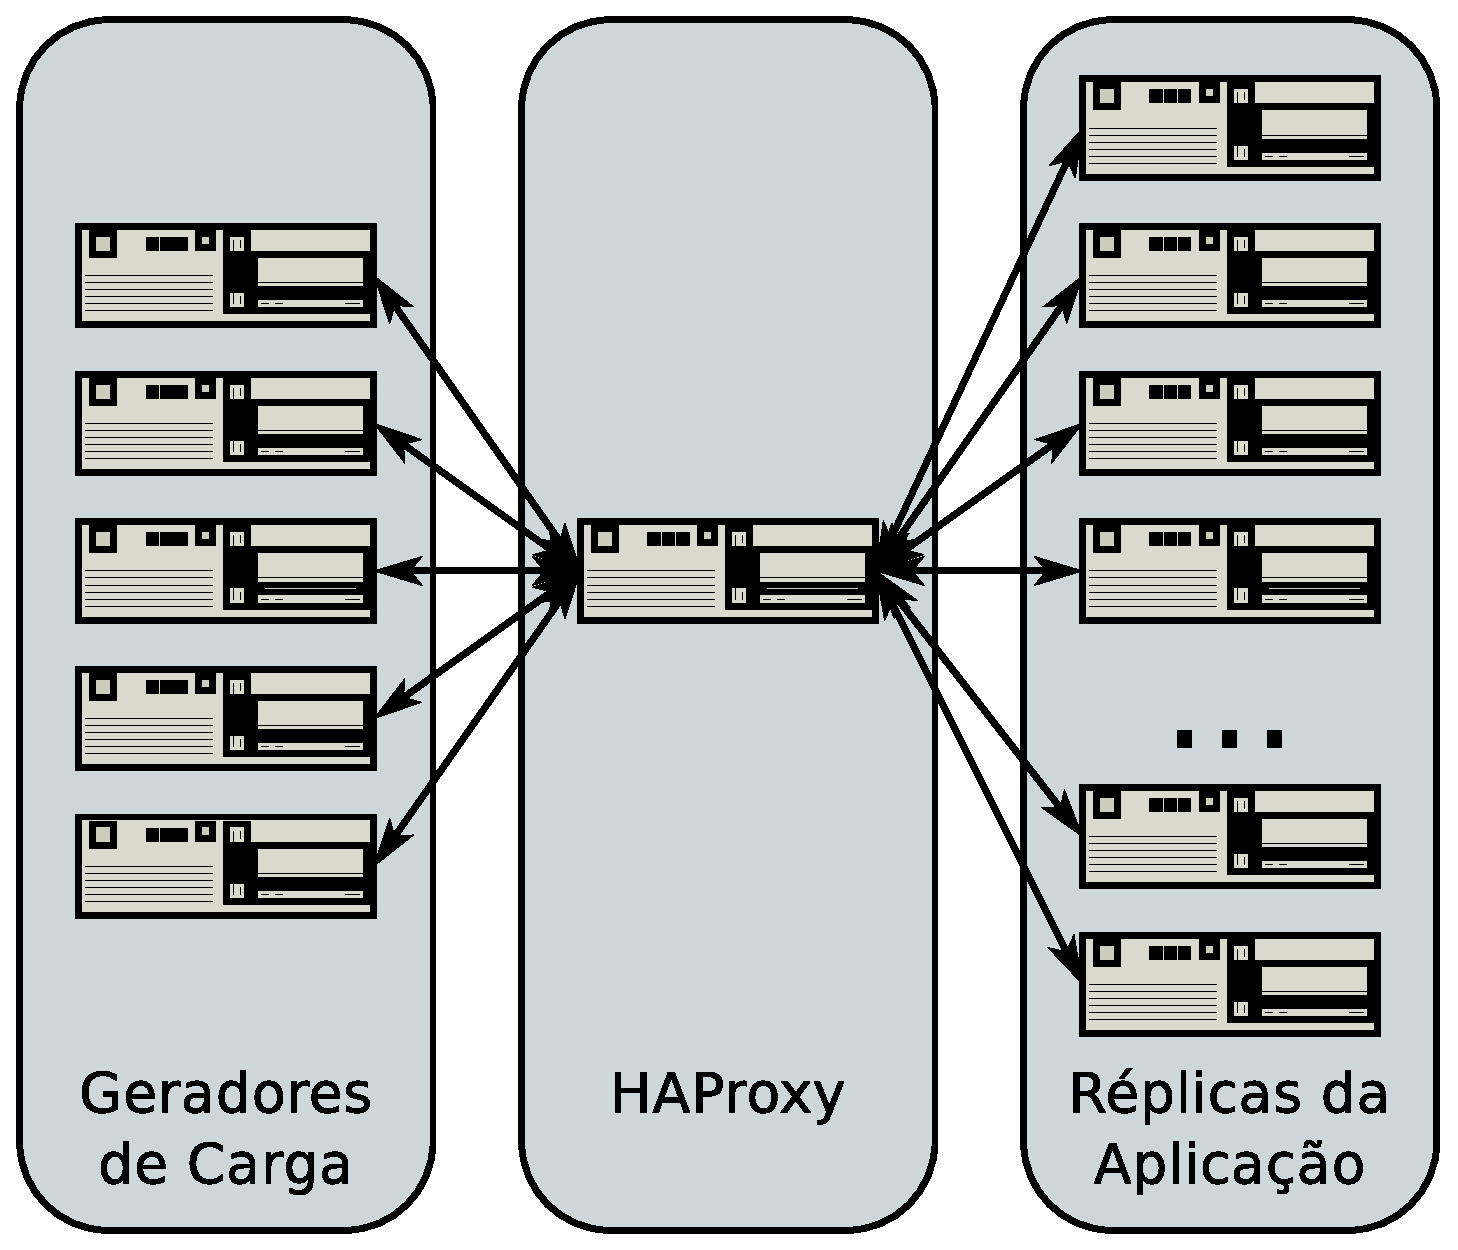
\includegraphics[width=7cm]{conteudo/capitulos/figuras/experimental-setup.dia.eps}
  \caption{Configuração experimental}
  \label{fig:setup}
\end{figure}

\subsection{Carga}

\subsubsection{Geração da carga}

\section{Experimento Transferência de Estado}\label{sec:experimento_tranferencia_estado}

\fbox{\begin{minipage}
  Lorem ipsum dolor sit amet, his at eruditi civibus. Mei mucius labores delicata ut,
  fuisset qualisque ut sea, pro invidunt theophrastus ei. Alterum accusam usu ex, id duo
  verear sapientem. Pro velit minim oblique et, diam meis ea usu. Per at tantas deserunt,
  lorem laboramus ca vel. Lobortis concludaturque mel ex, at liber viderer delicatissimi
  eos, eu vel altera sadipscing. Ad cum unum posse urbanitas. Vim idque hendrerit cu, homero
  bonorum omittam cu pro. Idque doming eu his, his te alias hinc.
\end{minipage}}

Cenários, carga, servidores

Resultados

Análise

\section{Experimento Elástico}\label{sec:experimento:replicas_leitoras}

Cenários, carga, servidores

Resultados

Análise


Descrever a proposta e sua implementação.


\include{conteudo/capitulos/capitulo_4}
\chapter*[Conclusão]{Conclusão}
\addcontentsline{toc}{chapter}{Conclusão}

Coloque o texto aqui.


\section*{Publicações}


\section*{Submissões}



% ----------------------------------------------------------

% ----------------------------------------------------------
% ELEMENTOS POS-TEXTUAIS
% ----------------------------------------------------------
\postextual
% ----------------------------------------------------------

% ----------------------------------------------------------
% Referencias bibliograficas
% ----------------------------------------------------------
\bibliography{referencias}


% ----------------------------------------------------------
% Glossario
% ----------------------------------------------------------
%
% Consulte o manual da classe abntex2 para orientacoes sobre o glossario.
%
%\glossary

% ----------------------------------------------------------
% Apendices
% ----------------------------------------------------------

% ---
% Inicia os apendices
% ---
%\begin{apendicesenv}

%\chapter{Título}\label{apendice1}

Texto ou documento elaborado pelo autor, a fim de complementar sua dissertação/argumentação.

%\end{apendicesenv}
% ---

% ----------------------------------------------------------
% Anexos
% ----------------------------------------------------------

% ---
% Inicia os anexos
% ---
%\begin{anexosenv}

%\chapter{Título}\label{anexo1}

Texto ou documento não elaborado pelo autor, que serve de fundamentação, comprovação e ilustração.

%\end{anexosenv}
% ---

%---------------------------------------------------------------------
% INDICE REMISSIVO
%---------------------------------------------------------------------
\phantompart
\printindex
%---------------------------------------------------------------------

\end{document}
